\documentclass[11pt,fleqn, openany]{book} % Default font size and left-justified equations

%%%%%%%%%%%%%%%%%%%%%%%%%%%%%%%%%%%%%%%%%
% The Legrand Orange Book
% Structural Definitions File
% Version 2.1 (26/09/2018)
%
% Original author:
% Mathias Legrand (legrand.mathias@gmail.com) with modifications by:
% Vel (vel@latextemplates.com)
% 
% This file was downloaded from:
% http://www.LaTeXTemplates.com
%
% License:
% CC BY-NC-SA 3.0 (http://creativecommons.org/licenses/by-nc-sa/3.0/)
%
%%%%%%%%%%%%%%%%%%%%%%%%%%%%%%%%%%%%%%%%%

%----------------------------------------------------------------------------------------
%	VARIOUS REQUIRED PACKAGES AND CONFIGURATIONS
%----------------------------------------------------------------------------------------

\usepackage[table]{xcolor}

\usepackage{graphicx}
\usepackage{tabularx} % Required for including pictures
\usepackage{pgf,tikz,tkz-tab,eurosym,yhmath, stmaryrd}
\usepackage{pgfplots}
\usepackage{mathrsfs}
\usetikzlibrary{patterns}
\usetikzlibrary{trees}
\graphicspath{{../../Pictures/}}
\usepackage{multicol} 


\usepackage[english]{babel} % English language/hyphenation
\usepackage{icomma}
\usepackage{enumitem} % Customize lists
\setlist{nolistsep, nosep, nolistsep} % Reduce spacing between bullet points and numbered lists

\usepackage{booktabs} % Required for nicer horizontal rules in tables

 % Required for specifying colors by name


\definecolor{ocre}{RGB}{243,102,25} % Define the orange color used for highlighting throughout the book

\usepackage{listings}

\definecolor{codegreen}{rgb}{0,0.6,0}
\definecolor{codegray}{rgb}{0.5,0.5,0.5}
\definecolor{codepurple}{rgb}{0.58,0,0.82}
\definecolor{backcolour}{rgb}{0.95,0.95,0.92}

\lstdefinestyle{mystyle}{
    backgroundcolor=\color{backcolour},   
    commentstyle=\color{codegreen},
    keywordstyle=\color{magenta},
    numberstyle=\tiny\color{codegray},
    stringstyle=\color{codepurple},
    basicstyle=\ttfamily\footnotesize,
    breakatwhitespace=false,         
    breaklines=true,                 
    captionpos=b,                    
    keepspaces=true,                 
    numbers=left,                    
    numbersep=5pt,                  
    showspaces=false,                
    showstringspaces=false,
    showtabs=false,                  
    tabsize=2
}

\lstset{style=mystyle}

%----------------------------------------------------------------------------------------
% Paramétrage XSIM
%----------------------------------------------------------------------------------------

\usepackage[no-files]{xsim}


\DeclareExerciseEnvironmentTemplate{myex}{%
    \textbf{%
      \hypertarget{ex:\ExerciseID}{\sffamily{\ensuremath{\blacktriangleright}} Exercice \GetExerciseProperty{counter} \GetExerciseProperty{subtitle} --}
      \hyperlink{sol:\ExerciseID}{Voir le corrigé}%
    }\par
}{\par\smallskip}

\DeclareExerciseEnvironmentTemplate{mysol}{%
    \textbf{%
      \hypertarget{sol:\ExerciseID}{\sffamily{\ensuremath{\blacktriangleright}} Correction \GetExerciseProperty{counter} --}
      \hyperlink{ex:\ExerciseID}{Voir l'énoncé}%
    }\par
}{\par\medskip}

\xsimsetup{
  exercise/template = myex ,
  solution/template = mysol 
}

%Collection exercices

\DeclareExerciseTagging{topic}

\xsimsetup{collect}

%----------------------------------------------------------------------------------------
% SYMBOLES
%----------------------------------------------------------------------------------------

\newcommand\imCMsym[4][\mathord]{%
  \DeclareFontFamily{U} {#2}{}
  \DeclareFontShape{U}{#2}{m}{n}{
    <-6> #25
    <6-7> #26
    <7-8> #27
    <8-9> #28
    <9-10> #29
    <10-12> #210
    <12-> #212}{}
  \DeclareSymbolFont{CM#2} {U} {#2}{m}{n}
  \DeclareMathSymbol{#4}{#1}{CM#2}{#3}
}
\newcommand\alsoimCMsym[4][\mathord]{\DeclareMathSymbol{#4}{#1}{CM#2}{#3}}

\imCMsym{cmmi}{124}{\CMjmath}

\newcommand{\Oij}{(O\,;\,\vec{\imath}\,,\, \vec{\CMjmath} )}
\newcommand{\Oijk}{(O\,;\,\vec{\imath}\,,\, \vec{\CMjmath}\,,\,\vec{k})}

\newcommand\e{\mathrm{e}}
\newcommand\R{\mathbb{R}}
\newcommand\N{\mathbb{N}}


%----------------------------------------------------------------------------------------
%	MARGINS
%----------------------------------------------------------------------------------------

\usepackage{geometry} % Required for adjusting page dimensions and margins

\geometry{
	paper=a4paper, % Paper size, change to letterpaper for US letter size
	top=3cm, % Top margin
	bottom=3cm, % Bottom margin
	left=2cm, % Left margin
	right=2cm, % Right margin
	headheight=14pt, % Header height
	footskip=1.4cm, % Space from the bottom margin to the baseline of the footer
	headsep=10pt, % Space from the top margin to the baseline of the header
	%showframe, % Uncomment to show how the type block is set on the page
}

\setlength{\parindent}{0pt}
\parskip=5pt



%----------------------------------------------------------------------------------------
%	FONTS
%----------------------------------------------------------------------------------------

\usepackage{avant} % Use the Avantgarde font for headings
\usepackage{times} % Use the Times font for headings
\usepackage{mathptmx} % Use the Adobe Times Roman as the default text font together with math symbols from the Sym­bol, Chancery and Com­puter Modern fonts

%\usepackage{microtype} % Slightly tweak font spacing for aesthetics
%\usepackage[utf8]{inputenc} % Required for including letters with accents
\usepackage[T1]{fontenc} % Use 8-bit encoding that has 256 glyphs

%----------------------------------------------------------------------------------------
%	BIBLIOGRAPHY AND INDEX
%----------------------------------------------------------------------------------------

\usepackage[style=numeric,citestyle=numeric,sorting=nyt,sortcites=true,autopunct=true,babel=hyphen,hyperref=true,abbreviate=false,backref=true,backend=biber]{biblatex}
\addbibresource{bibliography.bib} % BibTeX bibliography file
\defbibheading{bibempty}{}

\usepackage{calc} % For simpler calculation - used for spacing the index letter headings correctly
\usepackage{makeidx} % Required to make an index
\makeindex % Tells LaTeX to create the files required for indexing

%----------------------------------------------------------------------------------------
%	MAIN TABLE OF CONTENTS
%----------------------------------------------------------------------------------------

\usepackage{titletoc} % Required for manipulating the table of contents

\contentsmargin{0cm} % Removes the default margin

% Part text styling (this is mostly taken care of in the PART HEADINGS section of this file)
\titlecontents{part}
	[0cm] % Left indentation
	{\addvspace{20pt}\bfseries} % Spacing and font options for parts
	{}
	{}
	{}

% Chapter text styling
\titlecontents{chapter}
	[1.25cm] % Left indentation
	{\addvspace{12pt}\large\sffamily\bfseries} % Spacing and font options for chapters
	{\color{ocre!60}\contentslabel[\Large\thecontentslabel]{1.25cm}\color{ocre}} % Formatting of numbered sections of this type
	{\color{ocre}} % Formatting of numberless sections of this type
	{\color{ocre!60}\normalsize\;\titlerule*[.5pc]{.}\;\thecontentspage} % Formatting of the filler to the right of the heading and the page number

% Section text styling
\titlecontents{section}
	[1.25cm] % Left indentation
	{\addvspace{3pt}\sffamily\bfseries} % Spacing and font options for sections
	{\contentslabel[\thecontentslabel]{1.25cm}} % Formatting of numbered sections of this type
	{} % Formatting of numberless sections of this type
	{\hfill\color{black}\thecontentspage} % Formatting of the filler to the right of the heading and the page number

% Subsection text styling
\titlecontents{subsection}
	[1.25cm] % Left indentation
	{\addvspace{1pt}\sffamily\small} % Spacing and font options for subsections
	{\contentslabel[\thecontentslabel]{1.25cm}} % Formatting of numbered sections of this type
	{} % Formatting of numberless sections of this type
	{\ \titlerule*[.5pc]{.}\;\thecontentspage} % Formatting of the filler to the right of the heading and the page number

% Figure text styling
\titlecontents{figure}
	[1.25cm] % Left indentation
	{\addvspace{1pt}\sffamily\small} % Spacing and font options for figures
	{\thecontentslabel\hspace*{1em}} % Formatting of numbered sections of this type
	{} % Formatting of numberless sections of this type
	{\ \titlerule*[.5pc]{.}\;\thecontentspage} % Formatting of the filler to the right of the heading and the page number

% Table text styling
\titlecontents{table}
	[1.25cm] % Left indentation
	{\addvspace{1pt}\sffamily\small} % Spacing and font options for tables
	{\thecontentslabel\hspace*{1em}} % Formatting of numbered sections of this type
	{} % Formatting of numberless sections of this type
	{\ \titlerule*[.5pc]{.}\;\thecontentspage} % Formatting of the filler to the right of the heading and the page number

%----------------------------------------------------------------------------------------
%	MINI TABLE OF CONTENTS IN PART HEADS
%----------------------------------------------------------------------------------------

% Chapter text styling
\titlecontents{lchapter}
	[0em] % Left indentation
	{\addvspace{15pt}\large\sffamily\bfseries} % Spacing and font options for chapters
	{\color{ocre}\contentslabel[\Large\thecontentslabel]{1.25cm}\color{ocre}} % Chapter number
	{}  
	{\color{ocre}\normalsize\sffamily\bfseries\;\titlerule*[.5pc]{.}\;\thecontentspage} % Page number

% Section text styling
\titlecontents{lsection}
	[0em] % Left indentation
	{\sffamily\small} % Spacing and font options for sections
	{\contentslabel[\thecontentslabel]{1.25cm}} % Section number
	{}
	{}

% Subsection text styling (note these aren't shown by default, display them by searchings this file for tocdepth and reading the commented text)
\titlecontents{lsubsection}
	[.5em] % Left indentation
	{\sffamily\footnotesize} % Spacing and font options for subsections
	{\contentslabel[\thecontentslabel]{1.25cm}}
	{}
	{}

%----------------------------------------------------------------------------------------
%	HEADERS AND FOOTERS
%----------------------------------------------------------------------------------------


\usepackage{fancyhdr} % Required for header and footer configuration

\pagestyle{fancy}
\renewcommand{\chaptermark}[1]{\markboth{\sffamily\normalsize\bfseries\ \thechapter.\ #1}{}} % Chapter text font settings
\renewcommand{\sectionmark}[1]{\markright{\sffamily\normalsize\thesection\hspace{5pt}#1}{}} % Section text font settings
\fancyhf{} \fancyhead[LE,RO]{\sffamily\normalsize\thepage} % Font setting for the page number in the header
\fancyhead[LO]{\rightmark} % Print the nearest section name on the left side of odd pages
\fancyhead[RE]{\leftmark} % Print the current chapter name on the right side of even pages

\fancyfoot[L]{Jason LAPEYRONNIE}
\fancyfoot[R]{\href{http://mathoutils.fr}{http://mathoutils.fr}} % Uncomment to include a footer

\renewcommand{\headrulewidth}{0.5pt} % Thickness of the rule under the header
\renewcommand{\footrulewidth}{0.5pt} % Thickness of the rule under the header

\fancypagestyle{plain}{% Style for when a plain pagestyle is specified
	\fancyhead{}\renewcommand{\headrulewidth}{0pt}%
}

% Removes the header from odd empty pages at the end of chapters
\makeatletter
\renewcommand{\cleardoublepage}{
\clearpage\ifodd\c@page\else
\hbox{}
\vspace*{\fill}
\thispagestyle{empty}
\newpage
\fi}

%----------------------------------------------------------------------------------------
%	THEOREM STYLES
%----------------------------------------------------------------------------------------

\usepackage{amsmath,amsfonts,amssymb,amsthm} % For math equations, theorems, symbols, etc

\newcommand{\intoo}[2]{\mathopen{]}#1\,;#2\mathclose{[}}
\newcommand{\ud}{\mathop{\mathrm{{}d}}\mathopen{}}
\newcommand{\intff}[2]{\mathopen{[}#1\,;#2\mathclose{]}}
\renewcommand{\qedsymbol}{$\blacksquare$}
\newtheorem{notation}{Notation}[section]

% Boxed/framed environments
\newtheoremstyle{ocrenumbox}% Theorem style name
{0pt}% Space above
{0pt}% Space below
{\normalfont}% Body font
{}% Indent amount
{\small\bf\sffamily\color{ocre}}% Theorem head font
{\;:\;}% Punctuation after theorem head
{0.25em}% Space after theorem head
{\small\sffamily\color{ocre}\thmname{#1}\nobreakspace\thmnumber{\@ifnotempty{#1}{}\@upn{#2}}% Theorem text (e.g. Theorem 2.1)
\thmnote{\nobreakspace\the\thm@notefont\sffamily\bfseries\color{black}---\nobreakspace#3}} % Optional theorem note

\newtheoremstyle{blacknumex}% Theorem style name
{5pt}% Space above
{10pt}% Space below
{\normalfont}% Body font
{} % Indent amount
{\small\bf\sffamily}% Theorem head font
{\;:\;}% Punctuation after theorem head
{0.25em}% Space after theorem head
{\small\sffamily{\tiny\ensuremath{\blacksquare}}\nobreakspace\thmname{#1}\nobreakspace\thmnumber{\@ifnotempty{#1}{}\@upn{#2}}% Theorem text (e.g. Theorem 2.1)
\thmnote{\nobreakspace\the\thm@notefont\sffamily\bfseries---\nobreakspace#3}}% Optional theorem note

\newtheoremstyle{blacknumexo}% Theorem style name
{15pt}% Space above
{10pt}% Space below
{\normalfont}% Body font
{} % Indent amount
{\small\bf\sffamily}% Theorem head font
{}% Punctuation after theorem head
{0.5em}% Space after theorem head
{\small\sffamily{\ensuremath{\blacktriangleright}}\nobreakspace\thmname{#1}\nobreakspace\thmnumber{\@ifnotempty{#1}{}\@upn{#2}}% Theorem text (e.g. Theorem 2.1)
\thmnote{\nobreakspace\the\thm@notefont\sffamily\bfseries---\nobreakspace#3} \\}% Optional theorem note



\newtheoremstyle{blacknumbox} % Theorem style name
{0pt}% Space above
{5pt}% Space below
{}% Body font
{}% Indent amount
{\large\bf\sffamily}% Theorem head font
{\;:\;}% Punctuation after theorem head
{0.25em}% Space after theorem head
{\small\sffamily\thmname{#1}\nobreakspace\thmnumber{\@ifnotempty{#1}{}\@upn{#2}}% Theorem text (e.g. Theorem 2.1)
\thmnote{\nobreakspace\the\thm@notefont\sffamily\bfseries---\nobreakspace#3}}% Optional theorem note

% Non-boxed/non-framed environments
\newtheoremstyle{ocrenum}% Theorem style name
{5pt}% Space above
{5pt}% Space below
{\normalfont}% Body font
{}% Indent amount
{\small\bf\sffamily\color{ocre}}% Theorem head font
{\;:\;}% Punctuation after theorem head
{0.25em}% Space after theorem head
{\small\sffamily\color{ocre}\thmname{#1}\nobreakspace\thmnumber{\@ifnotempty{#1}{}\@upn{#2}}% Theorem text (e.g. Theorem 2.1)
\thmnote{\nobreakspace\the\thm@notefont\sffamily\bfseries\color{black}---\nobreakspace#3}} % Optional theorem note
\makeatother

% Defines the theorem text style for each type of theorem to one of the three styles above
\newcounter{dummy} 
\newcounter{thm}
\newcounter{correction}
\newcounter{qst}
\theoremstyle{ocrenumbox}
\newtheorem{theoremeT}[dummy]{Théorème}
\newtheorem{exerciseT}{Propriété}
\newtheorem{principeT}{Principe}
\theoremstyle{blacknumex}
\newtheorem{exampleT}{Exemple}
\theoremstyle{blacknumexo}
\newtheorem{exo}[thm]{Exercice}
\newtheorem{corr}[correction]{Correction}
\newtheorem{quest}[qst]{Question}
\theoremstyle{blacknumbox}
\newtheorem{vocabulary}{Vocabulary}[section]
\newtheorem{definitionT}{Définition}
\newtheorem{corollaryT}[dummy]{Corollary}
\theoremstyle{ocrenum}
\newtheorem{proofT}[dummy]{Démonstration}


%----------------------------------------------------------------------------------------
%	DEFINITION OF COLORED BOXES
%----------------------------------------------------------------------------------------

\RequirePackage[framemethod=default]{mdframed} % Required for creating the theorem, definition, exercise and corollary boxes

% Theorem box
\newmdenv[skipabove=7pt,
skipbelow=7pt,
backgroundcolor=black!5,
linecolor=ocre,
innerleftmargin=5pt,
innerrightmargin=5pt,
innertopmargin=10pt,
leftmargin=0cm,
rightmargin=0cm,
innerbottommargin=5pt]{tBox}

%Proposition box	  
\newmdenv[skipabove=7pt,
skipbelow=7pt,
rightline=false,
leftline=true,
topline=false,
bottomline=false,
backgroundcolor=ocre!10,
linecolor=ocre,
innerleftmargin=5pt,
innerrightmargin=5pt,
innertopmargin=10pt,
innerbottommargin=3pt,
leftmargin=0cm,
rightmargin=0cm,
linewidth=4pt]{eBox}	

% Definition box
\newmdenv[skipabove=7pt,
backgroundcolor=ocre!4,
skipbelow=7pt,
rightline=false,
leftline=true,
topline=false,
bottomline=false,
linecolor=ocre,
innerleftmargin=5pt,
innerrightmargin=5pt,
innertopmargin=10pt,
leftmargin=0cm,
rightmargin=0cm,
linewidth=4pt,
innerbottommargin=5pt]{dBox}	

% Corollary box
\newmdenv[skipabove=7pt,
skipbelow=7pt,
rightline=false,
leftline=true,
topline=false,
bottomline=false,
linecolor=gray,
backgroundcolor=black!5,
innerleftmargin=5pt,
innerrightmargin=5pt,
innertopmargin=5pt,
leftmargin=0cm,
rightmargin=0cm,
linewidth=4pt,
innerbottommargin=5pt]{cBox}

\newmdenv[skipabove=7pt,
skipbelow=7pt,
backgroundcolor=black!5,
innerleftmargin=5pt,
topline=false,
bottomline=false,
rightline=false,
leftline=false,
innerrightmargin=5pt,
innertopmargin=5pt,
leftmargin=0cm,
rightmargin=0cm,
innerbottommargin=5pt]{xBox}

% Creates an environment for each type of theorem and assigns it a theorem text style from the "Theorem Styles" section above and a colored box from above
\newenvironment{theorem}{\begin{tBox}\begin{theoremeT}}{\end{theoremeT}\end{tBox}}

\newenvironment{exo2}{\noindent \begin{exo}\item\relax \noindent \begin{eBox}\item\relax}{\end{eBox}\end{exo}}


\newenvironment{proposition}{\begin{eBox}\begin{exerciseT}}{\hfill{\color{ocre}}\end{exerciseT}\end{eBox}}		

\newenvironment{principe}{\begin{eBox}\begin{principeT}}{\hfill{\color{ocre}}\end{principeT}\end{eBox}}	
		  
\newenvironment{definition}{\begin{dBox}\begin{definitionT}}{\end{definitionT}\end{dBox}}	

\newenvironment{example}{\begin{xBox}\begin{exampleT}}{\hfill{\tiny\ensuremath{\blacksquare}}\end{exampleT}\end{xBox}}

\newenvironment{demonstration}{\begin{proofT}}{\hfill{\tiny\ensuremath{\square}}\end{proofT}}		
\newenvironment{corollary}{\begin{cBox}\begin{corollaryT}}{\end{corollaryT}\end{cBox}}	

%----------------------------------------------------------------------------------------
%	REMARK ENVIRONMENT
%----------------------------------------------------------------------------------------

\newenvironment{remark}{\par\vspace{5pt}\small % Vertical white space above the remark and smaller font size
\begin{list}{}{
\leftmargin=25pt % Indentation on the left
\rightmargin=15pt}\item\ignorespaces % Indentation on the right
\makebox[-2.5pt]{\begin{tikzpicture}[overlay]
\node[draw=ocre!60,line width=1pt,circle,fill=ocre!25,font=\sffamily\bfseries,inner sep=2pt,outer sep=0pt] at (-15pt,0pt){\textcolor{ocre}{R}};\end{tikzpicture}} % Orange R in a circle
\advance\baselineskip -1pt}{\end{list}\vskip5pt} % Tighter line spacing and white space after remark

%----------------------------------------------------------------------------------------
%	SECTION NUMBERING IN THE MARGIN
%----------------------------------------------------------------------------------------

\makeatletter
\renewcommand{\@seccntformat}[1]{\llap{\textcolor{ocre}{\csname the#1\endcsname}\hspace{1em}}}                    
\renewcommand{\section}{\@startsection{section}{1}{\z@}
{-4ex \@plus -1ex \@minus -.4ex}
{1ex \@plus.2ex }
{\normalfont\LARGE\sffamily\bfseries}}
\renewcommand{\subsection}{\@startsection {subsection}{2}{\z@}
{-3ex \@plus -0.1ex \@minus -.4ex}
{0.5ex \@plus.2ex }
{\normalfont\sffamily\bfseries}}
\renewcommand{\subsubsection}{\@startsection {subsubsection}{3}{\z@}
{-2ex \@plus -0.1ex \@minus -.2ex}
{.2ex \@plus.2ex }
{\normalfont\small\sffamily\bfseries}}                        
\renewcommand\paragraph{\@startsection{paragraph}{4}{\z@}
{-2ex \@plus-.2ex \@minus .2ex}
{.1ex}
{\normalfont\small\sffamily\bfseries}}

%----------------------------------------------------------------------------------------
%	PART HEADINGS
%----------------------------------------------------------------------------------------

% Numbered part in the table of contents
\newcommand{\@mypartnumtocformat}[2]{%
	\setlength\fboxsep{0pt}%
	\noindent\colorbox{ocre!20}{\strut\parbox[c][.7cm]{\ecart}{\color{ocre!70}\Large\sffamily\bfseries\centering#1}}\hskip\esp\colorbox{ocre!40}{\strut\parbox[c][.7cm]{\linewidth-\ecart-\esp}{\Large\sffamily\centering#2}}%
}

% Unnumbered part in the table of contents
\newcommand{\@myparttocformat}[1]{%
	\setlength\fboxsep{0pt}%
	\noindent\colorbox{ocre!40}{\strut\parbox[c][.7cm]{\linewidth}{\Large\sffamily\centering#1}}%
}

\newlength\esp
\setlength\esp{4pt}
\newlength\ecart
\setlength\ecart{1.2cm-\esp}
\newcommand{\thepartimage}{}%
\newcommand{\partimage}[1]{\renewcommand{\thepartimage}{#1}}%
\def\@part[#1]#2{%
\ifnum \c@secnumdepth >-2\relax%
\refstepcounter{part}%
\addcontentsline{toc}{part}{\texorpdfstring{\protect\@mypartnumtocformat{\thepart}{#1}}{\partname~\thepart\ ---\ #1}}
\else%
\addcontentsline{toc}{part}{\texorpdfstring{\protect\@myparttocformat{#1}}{#1}}%
\fi%
\startcontents%
\markboth{}{}%
{\thispagestyle{empty}%
\begin{tikzpicture}[remember picture,overlay]%
\node at (current page.north west){\begin{tikzpicture}[remember picture,overlay]%	
\fill[ocre!20](0cm,0cm) rectangle (\paperwidth,-\paperheight);
\node[anchor=north] at (4cm,-3.25cm){\color{ocre!40}\fontsize{220}{100}\sffamily\bfseries\thepart}; 
\node[anchor=south east] at (\paperwidth-1cm,-\paperheight+1cm){\parbox[t][][t]{8.5cm}{
\printcontents{l}{0}{\setcounter{tocdepth}{1}}% The depth to which the Part mini table of contents displays headings; 0 for chapters only, 1 for chapters and sections and 2 for chapters, sections and subsections
}};
\node[anchor=north east] at (\paperwidth-1.5cm,-3.25cm){\parbox[t][][t]{15cm}{\strut\raggedleft\color{white}\fontsize{30}{30}\sffamily\bfseries#2}};
\end{tikzpicture}};
\end{tikzpicture}}%
\@endpart}
\def\@spart#1{%
\startcontents%
\phantomsection
{\thispagestyle{empty}%
\begin{tikzpicture}[remember picture,overlay]%
\node at (current page.north west){\begin{tikzpicture}[remember picture,overlay]%	
\fill[ocre!20](0cm,0cm) rectangle (\paperwidth,-\paperheight);
\node[anchor=north east] at (\paperwidth-1.5cm,-3.25cm){\parbox[t][][t]{15cm}{\strut\raggedleft\color{white}\fontsize{30}{30}\sffamily\bfseries#1}};
\end{tikzpicture}};
\end{tikzpicture}}
\addcontentsline{toc}{part}{\texorpdfstring{%
\setlength\fboxsep{0pt}%
\noindent\protect\colorbox{ocre!40}{\strut\protect\parbox[c][.7cm]{\linewidth}{\Large\sffamily\protect\centering #1\quad\mbox{}}}}{#1}}%
\@endpart}
\def\@endpart{\vfil\newpage
\if@twoside
\if@openright
\null
\thispagestyle{empty}%
\newpage
\fi
\fi
\if@tempswa
\twocolumn
\fi}

%----------------------------------------------------------------------------------------
%	CHAPTER HEADINGS
%----------------------------------------------------------------------------------------

% A switch to conditionally include a picture, implemented by Christian Hupfer
\newif\ifusechapterimage
\usechapterimagetrue
\newcommand{\thechapterimage}{}%
\newcommand{\chapterimage}[1]{\ifusechapterimage\renewcommand{\thechapterimage}{#1}\fi}%
\newcommand{\autodot}{.}
\def\@makechapterhead#1{%
{\parindent \z@ \raggedright \normalfont
\ifnum \c@secnumdepth >\m@ne
\if@mainmatter
\begin{tikzpicture}[remember picture,overlay]
\node at (current page.north west)
{\begin{tikzpicture}[remember picture,overlay]
\node[anchor=north west,inner sep=0pt] at (0,0) {\ifusechapterimage\includegraphics[width=\paperwidth]{\thechapterimage}\fi};
\draw[anchor=west] (\Gm@lmargin,-3cm) node [line width=2pt,rounded corners=15pt,draw=ocre,fill=white,fill opacity=0.5,inner sep=15pt]{\strut\makebox[22cm]{}};
\draw[anchor=west] (\Gm@lmargin+.3cm,-3cm) node {\huge\sffamily\bfseries\color{black}\thechapter\autodot~#1\strut};
\end{tikzpicture}};
\end{tikzpicture}
\else
\begin{tikzpicture}[remember picture,overlay]
\node at (current page.north west)
{\begin{tikzpicture}[remember picture,overlay]
\node[anchor=north west,inner sep=0pt] at (0,0) {\ifusechapterimage\includegraphics[width=\paperwidth]{\thechapterimage}\fi};
\draw[anchor=west] (\Gm@lmargin,-3cm) node [line width=2pt,rounded corners=15pt,draw=ocre,fill=white,fill opacity=0.5,inner sep=15pt]{\strut\makebox[22cm]{}};
\draw[anchor=west] (\Gm@lmargin+.3cm,-3cm) node {\huge\sffamily\bfseries\color{black}#1\strut};
\end{tikzpicture}};
\end{tikzpicture}
\fi\fi\par\vspace*{50\p@}}}

%-------------------------------------------

\def\@makeschapterhead#1{%
\begin{tikzpicture}[remember picture,overlay]
\node at (current page.north west)
{\begin{tikzpicture}[remember picture,overlay]
\node[anchor=north west,inner sep=0pt] at (0,0) {\ifusechapterimage\includegraphics[width=\paperwidth]{\thechapterimage}\fi};
\draw[anchor=west] (\Gm@lmargin,-3cm) node [line width=2pt,rounded corners=15pt,draw=ocre,fill=white,fill opacity=0.5,inner sep=15pt]{\strut\makebox[22cm]{}};
\draw[anchor=west] (\Gm@lmargin+.3cm,-3cm) node {\huge\sffamily\bfseries\color{black}#1\strut};
\end{tikzpicture}};
\end{tikzpicture}
\par\vspace*{50\p@}}
\makeatother

%----------------------------------------------------------------------------------------
%	LINKS
%----------------------------------------------------------------------------------------

\usepackage{hyperref}
\hypersetup{hidelinks,backref=true,pagebackref=true,hyperindex=true,colorlinks=false,breaklinks=true,urlcolor=ocre,bookmarks=true,bookmarksopen=false}

\usepackage{bookmark}
\bookmarksetup{
open,
numbered,
addtohook={%
\ifnum\bookmarkget{level}=0 % chapter
\bookmarksetup{bold}%
\fi
\ifnum\bookmarkget{level}=-1 % part
\bookmarksetup{color=ocre,bold}%
\fi
}
}

\renewcommand*\thesection{\arabic{section}}

\newcommand*{\coord}[3]{% 
  \ensuremath{\overrightarrow{#1}\, 
    \begin{pmatrix} 
      #2\\ 
      #3 
    \end{pmatrix}}}
    
  \newcommand*{\coordb}[2]{% 
  \ensuremath{ 
    \begin{pmatrix} 
      #1\\ 
      #2 
    \end{pmatrix}}}

\newcommand*{\coorde}[4]{% 
  \renewcommand{\arraystretch}{1}\ensuremath{\overrightarrow{#1}\, 
    \begin{pmatrix} 
      #2\\ 
      #3 \\
      #4
    \end{pmatrix}}}    
  \newcommand*{\coordbe}[3]{% 
 \renewcommand{\arraystretch}{1} \ensuremath{ 
    \begin{pmatrix} 
      #1\\ 
      #2 \\
      #3
    \end{pmatrix}}}  
    
\newcommand{\Card}{\mathrm{Card}}


\begin{document}

\chapterimage{../../Pictures/background}

\chapter{Cours : Rappels de probabilité}



Avant de s'engager sur le programme de terminale, faisons quelques rappels de probabilités de l'année de Première.

Dans tout ce chapitre, on note $\Omega$ l'univers non vide d'une expérience aléatoire.\\
On rappelle que pour deux événements $A$ et $B$ de $\Omega$, l'événement $A \cap B$ est l'événement qui est réalisé lorsque « à la fois $A$ et $B$ sont réalisés ».\\De plus, l'événement $\bar{A}$, appelé contraire de $A$, est réalisé si et seulement si $A$ ne l'est pas.

$\mathbb{P}(A)$ désignera la probabilité de l'événement $A$. On a alors $\mathbb{P}(\overline{A})=1-\mathbb{P}(A)$.


\section{Probabilité conditionnelle}

\begin{definition}[Probabilité conditionnelle]Soit $A$ et $B$ deux événements tels que $\mathbb{P}(A)\neq 0$. On appelle probabilité conditionnelle de $B$ sachant $A$, la quantité
\[ \mathbb{P}_A(B)=\dfrac{\mathbb{P}(A\cap B)}{\mathbb{P}(A)}.\]\end{definition}

\begin{example} On considère l'univers $\Omega = \{ 1;2;3;4;5;6\}$. On tire un nombre uniformément au hasard sur $\Omega$. On  considère les événements
\begin{itemize}
\item $A$ : le nombre est pair ;
\item $B$ : le nombre est supérieur ou égal à 3.
\end{itemize}
Puisque l'on est en situation d'équiprobabilité, on a alors $\mathbb{P}(A)=\dfrac{3}{6}=\dfrac{1}{2}$ et $\mathbb{P}(B)=\dfrac{4}{6}=\dfrac{2}{3}$.\\
Par ailleurs, $A\cap B = \{4;6\}$. Ainsi, $\mathbb{P}(A \cap B) = \dfrac{2}{6}=\dfrac{1}{3}$.\\
Appliquant la définition, on trouve donc 
\[ \mathbb{P}_A(B)=\dfrac{\mathbb{P}(A\cap B)}{\mathbb{P}(A)}=\dfrac{\dfrac{1}{3}}{\dfrac{1}{2}}=\dfrac{2}{3}\quad
\text{et} 
\quad \mathbb{P}_B(A)=\dfrac{\mathbb{P}(B\cap A)}{\mathbb{P}(B)}=\dfrac{\dfrac{1}{3}}{\dfrac{2}{3}}=\dfrac{1}{2}.\]
\end{example}

Cette probabilité s'interprète comme la probabilité de l'événement $B$ sachant que l'événement $A$ est réalisé.

\begin{example}Une entreprise commande à une société de sondage une enquête sur la satisfaction de ses clients. Lors du premier appel téléphonique, la probabilité qu'un client réponde est de 0,25. Si le client répond à l'appel, la probabilité qu'il réponde au questionnaire de la société est de 0,3. On note $R$ l'événement « la personne répond à l'appel » et $Q$ l'événement « la personne répond au questionnaire ». 

D'après l'énoncé, on a $\mathbb{P}(R)=0,25$ et $\mathbb{P}_R(Q)=0,3$. Ainsi, la probabilité qu'une personne prise au hasard réponde à l'appel puis au questionnaire vaut $\mathbb{P}(R \cap Q) = \mathbb{P}(R) \times \mathbb{P}_R(Q)=0,3 \times 0,25 = 0,075$.\end{example}

\newpage

\subsection{Construction d'un arbre pondéré}

\begin{proposition}[Règle de la somme] Dans un arbre pondéré, la somme des probabilités issues d'un nœud est égale à 1.
\end{proposition}

\begin{example} On considère une succession de deux expériences aléatoires dont l'arbre pondéré associé est représenté ci-dessous.
\tikzstyle{level 1}=[level distance=3.5cm, sibling distance=4cm]
\tikzstyle{level 2}=[level distance=3.5cm, sibling distance=1.5cm]
\tikzstyle{level 3}=[level distance=3.5cm, sibling distance=0.3cm]

% Define styles for bags and leafs
\tikzstyle{bag} = [text width=4em, text centered]
\tikzstyle{end} = [circle, minimum width=3pt,fill, inner sep=0pt]


\begin{center}
\begin{tikzpicture}[scale=0.8,grow=right,sloped]
\node[bag] { }
    child {
        node[bag] {C} 
        child {
                node[bag] {F}
                edge from parent node[below] {$0.3$}
            }
        child {
               node[bag] {E}
               edge from parent node[above] {$0.4$}
            }
        child {
                node[bag] {D}
                edge from parent [very thick, red]
            }
            edge from parent node[above] {$0.6$} 
    }
    child {
        node[bag] {B}        
            child {
                node[bag] {F}
                edge from parent [black] node[below] {$0.2$}
            }
            child {
                node[bag] {E}
                 child{
                	node[bag] {$B\cap E$}
                	edge from parent [dashed,->]
                	}
                edge from parent [black] node[above] {$0.4$}
            }
            child {
                node[bag] {D}
                edge from parent [black] node[above] {$0.4$}
            }
            edge from parent [thick, blue]
    }
     child {
        node[bag] {A}        
            child {
                node[bag] {F}
                edge from parent node[below] {$0.1$}
            }
            child {
                node[bag] {E}
                edge from parent node[above] {$0.1$}
            }
            child {
                node[bag] {D}
                child{
                	node[bag] {$A\cap D$}
                	edge from parent [dashed,->]
                	}
                edge from parent node[above] {$0.8$}
            }
            edge from parent node[above] {$0.3$}
        };
\end{tikzpicture}
\end{center}



\begin{itemize}
\item Sur cet arbre, on voit que $\mathbb{P}(A)=0.3$ et $\mathbb{P}(C)=0.6$.
\item Puisque la somme des probabilités issues d'une branche vaut 1, on a $\mathbb{P}(A)+\mathbb{P}(B)+\mathbb{P}(C)=1$, soit $\mathbb{P}(B)=0.1$.
\item La probabilité conditionnelle $\mathbb{P}_A(D)$ se lit sur la branche qui relie $A$ à $D$. Ainsi, $\mathbb{P}_A(D)=0.8$.
\item La somme des probabilités issues du nœud $C$ doit valoir 1. \\ On a donc $\mathbb{P}_C(D)+\mathbb{P}_C(E)+\mathbb{P}_C(F)=1$. Ainsi, $\mathbb{P}_C(D)=0.3$.
\end{itemize}\end{example}

Cette règle traduit le fait que l'on construit l'arbre en découpant l'univers selon des événements disjoints. Ici, $A\cap B = \varnothing$.

\begin{proposition}[Règle du produit] Dans un arbre pondéré la probabilité d'une issue est égale au produit des probabilités du chemin aboutissant à cette issue
\end{proposition}

\begin{example}Pour obtenir l'issue $A\cap D$, on passe par les sommets $A$ puis $D$.

On a alors $\mathbb{P}(A\cap D)=0.3 \times 0.8=0.24$.\end{example}

On retrouve la relation $\mathbb{P}(A \cap D)= \mathbb{P}(A) \times \mathbb{P}_A(D)$.
\newpage
\subsection{Formule des probabilités totales}

\begin{definition}[Partition]Soit $\Omega$ l'univers d'une expérience aléatoire. \\On dit que les événements $A_1$, $A_2$, ..., $A_n$ forment une partition de $\Omega$ lorsque
\begin{itemize}
\item Les ensembles $A_1$, $A_2$, ..., $A_n$ sont non vides ;
\item Les ensembles $A_1$, $A_2$, ..., $A_n$ sont deux à deux disjoints ;
\item $A_1\cup A_2\cup \ldots \cup A_n = \Omega$.
\end{itemize}
Dans le cadre des probabilités, on parle également de \textbf{système complet d'événements}.\end{definition}

\begin{example}On considère $\Omega = \{1;2;3;4;5;6;7;8\}$ ainsi que les événements $A_1=\{1;3\}$, \\ $A_2=\{2;4;5;6;7\}$ et $A_3=\{8\}$. $A_1$, $A_2$ et $A_3$ forment une partition de $\Omega$.\end{example}

\begin{proposition}[Formule des probabilités totales] On considère un événement $B$ et une partition $A_1$, $A_2$, ..., $A_n$ de l'univers $\Omega$. Alors,
\[ \mathbb{P}(B)=\mathbb{P}(B \cap A_1) + \mathbb{P}(B \cap A_2) + \ldots + \mathbb{P}(B \cap A_n) = \sum_{i=1}^{n} \mathbb{P}(B\cap A_i).\]
\end{proposition}


\begin{example} On reprend l'exemple de la partie précédente. On souhaite calculer la probabilité $\mathbb{P}(D)$. Pour cela, on regarde l'ensemble des branches qui contiennent l'événement $D$.

\tikzstyle{level 1}=[level distance=3.5cm, sibling distance=4cm]
\tikzstyle{level 2}=[level distance=3.5cm, sibling distance=1.5cm]
\tikzstyle{level 3}=[level distance=3.5cm, sibling distance=0.3cm]

% Define styles for bags and leafs
\tikzstyle{bag} = [text width=4em, text centered]
\tikzstyle{end} = [circle, minimum width=3pt,fill, inner sep=0pt]


\begin{center}
\begin{tikzpicture}[scale=0.7,grow=right,sloped]
\node[bag] { }
    child {
        node[bag] {C} 
        child {
                node[bag] {F}
                edge from parent node[below] {$0.3$}
            }
        child {
               node[bag] {E}
               edge from parent node[above] {$0.4$}
            }
        child {
                node[bag] {D}
                child{
                	node[bag] {$C\cap D$}
                	edge from parent [dashed,->]
                	}
                edge from parent node[above] {$0.3$}
            }
            edge from parent node[above] {$0.6$} 
    }
    child {
        node[bag] {B}        
            child {
                node[bag] {F}
                edge from parent [black] node[below] {$0.2$}
            }
            child {
                node[bag] {E}
                edge from parent [black] node[above] {$0.4$}
            }
            child {
                node[bag] {D}
                    child{
                	node[bag] {$B\cap D$}
                	edge from parent [dashed,->]
                	}
                edge from parent [black] node[above] {$0.4$}
            }
            edge from parent node[above] {$0.1$}
    }
     child {
        node[bag] {A}        
            child {
                node[bag] {F}
                edge from parent node[below] {$0.1$}
            }
            child {
                node[bag] {E}
                edge from parent node[above] {$0.1$}
            }
            child {
                node[bag] {D}
                child{
                	node[bag] {$A\cap D$}
                	edge from parent [dashed,->]
                	}
                edge from parent node[above] {$0.8$}
            }
            edge from parent node[above] {$0.3$}
        };
\end{tikzpicture}
\end{center}

\begin{itemize}
\item $A$, $B$ et $C$ forment une partition de $\Omega$.
\item On a $\mathbb{P}(D)=\mathbb{P}(A\cap D) + \mathbb{P}(B\cap D) + \mathbb{P}(C\cap D)$. De plus,
\begin{itemize}
\item $\mathbb{P}(A\cap D)=\mathbb{P}_A(D) \times \mathbb{P}(A)= 0.8 \times 0.3 = 0.24$ ;
\item $\mathbb{P}(B\cap D)=\mathbb{P}_B(D) \times \mathbb{P}(B)= 0.4 \times 0.1 = 0.04$ ;
\item $\mathbb{P}(C\cap D)=\mathbb{P}_C(D) \times \mathbb{P}(C)= 0.6 \times 0.3 = 0.18$.
\end{itemize}
\item Ainsi, $\mathbb{P}(D)=0.24+0.04+0.18=0.46$.
\end{itemize}
\vspace{-0.5cm}
\end{example}


\section{Variable aléatoire réelle}

\subsection{Variable aléatoire}

\begin{definition}On appelle variable aléatoire réelle toute fonction définie sur l'univers $\Omega$ d'une expérience aléatoire et à valeurs dans $\mathbb{R}$.\\
Les variables aléatoires sont en général notées $X$.\end{definition}

\begin{minipage}{0.55\linewidth}\begin{example}On choisit un nombre entier au hasard entre 1 et 6 compris. L'univers de l'expérience aléatoire est donc l'ensemble $\{1;2;3;4;5;6\}$.

Si le nombre obtenu est 6, on gagne 2 points. Si le nombre est impair, on perd 1 point. Dans les autres cas, on ne gagne ni ne perd aucun point.\\
On appelle $X$ la variable aléatoire qui donne le nombre de points gagnés selon le résultat.
\begin{itemize}
\item Si on obtient le nombre 1, on perd 1 point. \\On a ainsi $X(1)=-1$.
\item Si on obtient le nombre 6, on gagne 2 points. \\On a ainsi $X(6)=2$.
\item On a également $X(2)=0$, $X(3)=-1$, $X(4)=0$ et $X(5)=-1$.
\end{itemize}\end{example}
\end{minipage}\hfill\begin{minipage}{0.43\linewidth}

\tikzstyle{level 1}=[level distance=2.5cm, sibling distance=1.5cm]
\tikzstyle{level 2}=[level distance=4.2cm, sibling distance=1.5cm]
\tikzstyle{level 3}=[level distance=3.5cm, sibling distance=0.3cm]

% Define styles for bags and leafs
\tikzstyle{bag} = [text width=4em, text centered]
\tikzstyle{end} = [circle, minimum width=3pt,fill, inner sep=0pt]


\begin{center}
\begin{tikzpicture}[scale=0.8,grow=right,sloped]
\draw (3,5) node {\textbf{Univers}};
\draw (7,5) node {\textbf{Variable}};
\draw (7,4.8) node[below] {\textbf{aléatoire}};
\node[bag] { }
    child {
        node[bag] {6} 
        child {
                node[bag] {2}
                edge from parent[dashed,->,>=latex] node[below] {$ $}
            }
            edge from parent node[above] {$ $} 
    }
	child {
        node[bag] {5} 
        child {
                node[bag] {$-1$}
                edge from parent[dashed,->,>=latex] node[below] {$ $}
            }
            edge from parent node[above] {$ $} 
    }
    child {
        node[bag] {4} 
        child {
                node[bag] {0}
                edge from parent[dashed,->,>=latex] node[below] {$ $}
            }
            edge from parent node[above] {$ $} 
    }
    child {
        node[bag] {3} 
        child {
                node[bag] {$-1$}
                edge from parent[dashed,->,>=latex] node[below] {$ $}
            }
            edge from parent node[above] {$ $} 
    }
    child {
        node[bag] {2} 
        child {
                node[bag] {0}
                edge from parent[dashed,->,>=latex] node[below] {$ $}
            }
            edge from parent node[above] {$ $} 
    }
    child {
        node[bag] {1} 
        child {
                node[bag] {$-1$}
                edge from parent[dashed,->,>=latex] node[below] {$ $}
            }
            edge from parent node[above] {$ $} 
    }
    ;
\end{tikzpicture}
\end{center}\end{minipage}


\begin{definition}Soit $X$ une variable aléatoire réelle sur un univers $\Omega$ et $a$ un réel.\\
On note $\{X=a\}$ l'événement qui regroupe toutes les issues $\omega$ de $\Omega$ telle que $X(\omega)=a$.\\
On peut définir de la même manière les événements $\{X<a\}$, $\{X\leqslant a\}$, $\{X\geqslant a\}$...\end{definition}

\begin{example}On reprend l'exemple précédent.
\begin{itemize}
\item L'événement $\{X=-1\}$ correspond aux issues qui font perdre un point, soit les issues 1, 3 et 5.
\item L'événement $\{X\geqslant 0\}$ correspond aux issues qui font gagner 0 point ou plus, soit les issues 2, 4 et 6.
\end{itemize}\end{example}

\subsection{Loi d'une variable aléatoire}


\begin{definition}Soit $X$ une variable aléatoire réelle sur un univers fini $\Omega$.\\
La loi de probabilité de $X$ est la fonction qui, à chaque réel $k$, associe la probabilité  $\mathbb{P}(X=k)$.\end{definition}

On rappelle que \textbf{la somme des probabilités doit valoir 1} !

\begin{example}On choisit uniformément au hasard un nombre entier entre 1 et 8 compris.

\begin{itemize}
\item Si le nombre obtenu est supérieur ou égal à 6, on gagne 2 points.
\item Si le nombre obtenu est inférieur ou égal à 4, on perd 3 points.
\item Si le nombre obtenu est 5, on gagne 5 points.
\end{itemize}
On note $X$ la variable aléatoire qui donne le nombre de points gagnés après l'expérience.\\


\tikzstyle{level 1}=[level distance=3.5cm, sibling distance=1cm]
\tikzstyle{level 2}=[level distance=5cm, sibling distance=1.5cm]
\tikzstyle{level 3}=[level distance=3.5cm, sibling distance=0.3cm]

% Define styles for bags and leafs
\tikzstyle{bag} = [text width=4em, text centered]
\tikzstyle{end} = [circle, minimum width=3pt,fill, inner sep=0pt]


\begin{center}
\begin{tikzpicture}[scale=0.8,grow=right,sloped]
\draw (3.5,4.5) node {\textbf{Univers}};
\draw (8.5,4.5) node {\textbf{Variable aléatoire $X$}};
\node[bag] { }
	child {
        node[bag] {8} 
        child {
                node[bag] {$2$}
                edge from parent[dashed,->,>=latex] node[below] {$ $}
            }
            edge from parent node[above] {$ $} 
    }
    child {
        node[bag] {7} 
        child {
                node[bag] {$2$}
                edge from parent[dashed,->,>=latex] node[below] {$ $}
            }
            edge from parent node[above] {$ $} 
    }
    child {
        node[bag] {6} 
        child {
                node[bag] {2}
                edge from parent[dashed,->,>=latex] node[below] {$ $}
            }
            edge from parent node[above] {$ $} 
    }
	child {
        node[bag] {5} 
        child {
                node[bag] {$5$}
                edge from parent[dashed,->,>=latex] node[below] {$ $}
            }
            edge from parent node[above] {$ $} 
    }
    child {
        node[bag] {4} 
        child {
                node[bag] {$-3$}
                edge from parent[dashed,->,>=latex] node[below] {$ $}
            }
            edge from parent node[above] {$ $} 
    }
    child {
        node[bag] {3} 
        child {
                node[bag] {$-3$}
                edge from parent[dashed,->,>=latex] node[below] {$ $}
            }
            edge from parent node[above] {$ $} 
    }
    child {
        node[bag] {2} 
        child {
                node[bag] {$-3$}
                edge from parent[dashed,->,>=latex] node[below] {$ $}
            }
            edge from parent node[above] {$ $} 
    }
    child {
        node[bag] {1} 
        child {
                node[bag] {$-3$}
                edge from parent[dashed,->,>=latex] node[below] {$ $}
            }
            edge from parent node[above] {$1/8$} 
    }
    ;
\end{tikzpicture}
\end{center}

$X$ peut donc prendre trois valeurs : $-3$, $2$ ou $5$. Pour déterminer la loi de $X$, il faut donc déterminer $\mathbb{P}(X=-3)$, $\mathbb{P}(X=2)$ et $\mathbb{P}(X=5)$.
\begin{itemize}
\item L'événement $\{X=-3\}$ est composé des issues 1, 2, 3 et 4. \\ Puisque l'on est en situation d'équiprobabilité, $\mathbb{P}(X=-3)=\dfrac{4}{8}=\dfrac{1}{2}$.
\vskip5pt
\item L'événement $\{X=2\}$ est composé des issues 6, 7 et 8. \\ Puisque l'on est en situation d'équiprobabilité, $\mathbb{P}(X=2)=\dfrac{3}{8}$.
\vskip5pt
\item L'événement $\{X=5\}$ est composé de l'issue 5. \\ Puisque l'on est en situation d'équiprobabilité, $\mathbb{P}(X=-3)=\dfrac{1}{8}$.
\end{itemize}
On peut résumer la loi de la variable aléatoire $X$ dans un tableau.
\renewcommand{\arraystretch}{2.2}
\begin{center}
\begin{tabular}{|l|c|c|c|}
\hline
$k$ & $-3$ & $2$ & $5$ \\
\hline
$\mathbb{P}(X=k)$ & $\dfrac{1}{2}$ & $\dfrac{3}{8}$ & $\dfrac{1}{8}$ \\
\hline \end{tabular}
\end{center}
\end{example}


\subsection{Espérance d'une variable aléatoire réelle}

\begin{definition}Soit $X$ une variable aléatoire. On note $x_1$, $x_2$, ..., $x_n$ les valeurs prises par $X$.\\
Pour $i$ allant de $1$ à $n$, on note $p_i$ la probabilité $\mathbb{P}(X=x_i)$. L'espérance de $X$, notée $E[X]$, est la valeur
\[ E[X]= p_1x_1+p_2x_2+\ldots + p_n x_n = \sum _{i=1}^{n} p_i x_i.\]\end{definition}

Il s'agit en quelque sorte de la moyenne des valeurs prises par la variable aléatoire $X$, pondérées par leurs probabilités. Nous verrons dans un prochain chapitre que le terme de moyenne prendra tout son sens...
\newpage
\begin{example}On considère une variable aléatoire $X$ dont la loi est donnée par le tableau suivant.

\renewcommand{\arraystretch}{2.2}
\begin{center}
\begin{tabular}{|l|c|c|c|c|}
\hline
$k$ & $-1$& $2$ & $3$ & $8$ \\
\hline
$\mathbb{P}(X=k)$ & $\dfrac{1}{3}$ & $\dfrac{1}{4}$ & $\dfrac{1}{6}$ & $\dfrac{1}{4}$\\
\hline \end{tabular}
\end{center}


L'espérance de la variable aléatoire $X$ vaut :
\[ E[X]= \dfrac{1}{3} \times (-1) + \dfrac{1}{4} \times 2 + \dfrac{1}{6} \times 3 + \dfrac{1}{4} \times 8 = \dfrac{8}{3}.\]

« En moyenne », la variable aléatoire $X$ vaut $\dfrac{8}{3}$.\end{example}

\subsection{Variance et écart-type d'une variable aléatoire réelle}

\begin{definition}Soit $X$ une variable aléatoire. On note $x_1$, $x_2$, ..., $x_n$ les valeurs prises par la variable aléatoire $X$.
La variance $X$, notée $V(X)$, est la valeur
\[ V(X)= p_1(x_1-E[X])^2+p_2(x_2-E[X])^2+\ldots + p_n( x_n-E[X])^2 = \sum _{i=1}^{n} p_i (x_i-E[X])^2.\]
Cette quantité mesure la dispersion de la variable aléatoire autour de l'espérance.\end{definition}

\textbf{Remarque :} On a en fait $V(X)= E[ (X-E[X])^2 ]$.

\begin{example}On considère une variable aléatoire $X$ dont la loi est donnée par le tableau suivant.

\renewcommand{\arraystretch}{2.2}
\begin{center}
\begin{tabular}{|l|c|c|c|c|}
\hline
$k$ & $-3$& $1$ & $4$ & $9$ \\
\hline
$\mathbb{P}(X=k)$ & $0.6$ & $0.2$ & $0.15$ & $0.05$\\
\hline \end{tabular}
\end{center}

Dans un premier temps, on calcule l'espérance de la variable aléatoire $X$.
\[E[X] = -3 \times 0.6 + 1 \times 0.2 + 4 \times 0.15 + 9 \times 0.05=-0.55.\]

Pour calculer la variance,
\begin{itemize}
\item Pour chaque valeur de la variable aléatoire, on retire l'espérance. On dit que l'on centre la variable aléatoire ;
\item On met chaque nombre obtenu au carré ;
\item Chaque nombre est multiplié par sa probabilité ;
\item On ajoute alors chacun des nombres obtenus.
\end{itemize}
\newpage
Dans ce cas,
\renewcommand{\arraystretch}{2.2}
\begin{center}
\begin{tabular}{|l|c|c|c|c|}
\hline
$x_i$ & $-3$& $1$ & $4$ & $9$ \\
\hline
$x_i-E[X]$ & $-2.45$ & $1.55$ & $4.55$ & $9.55$ \\
\hline
$(x_i-E[X])^2$ & $6.0025$ & $2.4025$ & $20.7025$ & $91.2025$\\
\hline
$p_i$ & $0.6$ & $0.2$ & $0.15$ & $0.05$\\
\hline
$p_i(x_i-E[X])^2$ & $3.6015$ & $0.4805$ & $3.105375$ & $4.560125$\\
\hline \end{tabular}
\end{center}

La variance de $X$ vaut donc 
\[ V(X) = 3.6015+0.4805+3.105375+4.560125=11.7475 .\]\end{example}

\begin{proposition}[Formule de König-Huygens]
Soit $X$ une variable aléatoire. On a alors
\[V(X)=E[X^2]-(E[X])^2.\]
\end{proposition}

\begin{example}
Reprenons l'exemple précédent. Pour déterminer la loi de $X^2$, il suffit de mettre les valeurs prises par la variable aléatoire au carré. On a alors

\renewcommand{\arraystretch}{2.2}
\begin{center}
\begin{tabular}{|l|c|c|c|c|}
\hline
$k$ & $9$& $1$ & $16$ & $81$ \\
\hline
$\mathbb{P}(X^2=k)$ & $0.6$ & $0.2$ & $0.15$ & $0.05$\\
\hline \end{tabular}
\end{center}

Ainsi, $E[X^2]=9 \times 0.6 +1 \times 0.2+16 \times 0.15+81 \times 0.05=12.05$.

On a donc $V(X)=E[X^2]-(E[X])^2=12.05-(-0.55)^2=11.7475$. On retrouve bien la valeur précédente.

\end{example}

\begin{definition} Soit $X$ une variable aléatoire réelle. On appelle écart-type de $X$, noté $\sigma(X)$ (sigma), la valeur
\[ \sigma (X)= \sqrt{V(X)}.\]\end{definition}

L'écart-type mesure la "variation moyenne" de la variable aléatoire autour de l'espérance.

\begin{example}Dans l'exemple précédent, l'écart-type était donc $\sigma(X)=\sqrt{11.7475}\simeq 3.42$.\end{example}

\chapter{Exercices}

\section*{Probabilités conditionnelles}

\begin{exercise}[subtitle={(Polynésie 2021)}]

Un test est mis au point pour détecter une maladie dans un pays.
Selon les autorités sanitaires de ce pays, 7\% des habitants sont infectés par cette maladie. Parmi les individus infectés, 20\% sont déclarés négatifs.
Parmi les individus sains, 1\% sont déclarés positifs.
Une personne est choisie au hasard dans la population.

On note
\begin{itemize}
\item $M$ l'événement : « la personne est infectée par la maladie » ;
\item $T$ l'événement : « le test est positif ».
\end{itemize}

\begin{enumerate}
\item Construire un arbre pondéré modélisant la situation.
\item \begin{enumerate}
\item Quelle est la probabilité pour que la personne soit infectée et que son test soit positif ?
\item Montrer que la probabilité que son test soit positif est de $0,0653$.
\end{enumerate}
\item On sait que le test de la personne choisie est positif. Quelle est la probabilité qu'elle soit infectée ?
On donnera le résultat sous forme approchée à $10^{-2}$ près.
\end{enumerate}

\end{exercise}
\begin{solution}\hspace{0pt}

\begin{enumerate}

\item On construit l'arbre pondéré suivant.

\tikzstyle{level 1}=[level distance=3.5cm, sibling distance=3cm]
\tikzstyle{level 2}=[level distance=3.5cm, sibling distance=1.5cm]
\tikzstyle{level 3}=[level distance=3.5cm, sibling distance=0.3cm]

% Define styles for bags and leafs
\tikzstyle{bag} = []
\tikzstyle{end} = [circle, minimum width=3pt,fill, inner sep=0pt]


\begin{center}
\begin{tikzpicture}[scale=0.8,grow=right,sloped]
\node[bag] { }
	child {
        node[bag] {$\overline{M}$} 
        child {
                node[bag] {$\overline{T}$}
                edge from parent node[below] {$0.99$}
            }
        child {
               node[bag] {$T$}
               edge from parent node[above] {$0.01$}
            }
            edge from parent node[below] {$0.93$}
    }
	child {
        node[bag] {$M$} 
        child {
                node[bag] {$\overline{T}$}
                edge from parent node[below] {$0.2$}
            }
        child {
               node[bag] {$T$}
               edge from parent node[above] {$0.8$}
            }
            edge from parent node[above] {$0.07$}
    };
\end{tikzpicture}
\end{center}

\item \begin{enumerate}
\item La probabilité pour que la personne soit infectée et que son test soit positif est $\mathbb{P}(M \cap T)$. 

Cette probabilité vaut $\mathbb{P}(M) \times \mathbb{P}_M(T)$ soit $0.07 \times 0.8$ soit $0.056$.
\item $(M;\overline{M})$ forme un système complet d'événements. D'après la formule des probabilités totales
\[\mathbb{P}(T)=\mathbb{P}(M \cap T)+\mathbb{P}(\overline{M} \cap T)=0.056+0.93 \times 0.01 = 0.0653.\]
\end{enumerate}
\item On a $\mathbb{P}_T(M)=\dfrac{\mathbb{P}(M\cap T)}{\mathbb{P}(T)}=\dfrac{0.056}{0.0653}\simeq 0.86$. La probabilité qu'une personne dont le test est positif soit infectée est d'environ 0,86.
\end{enumerate}

\end{solution}





\begin{exercise}[subtitle={(Centres étrangers 2021)}]

D'après une étude, les utilisateurs réguliers de transports en commun représentent 17\% de la population française. Parmi ces utilisateurs réguliers, 32\% sont des jeunes âgés  de 18 à 24 ans.

On interroge une personne au hasard et on note :
\begin{itemize}
\item $R$ : « La personne interrogée utilise régulièrement les transports en commun » ;
\item $J$ : « La personne interrogée est âgée de 18 à 24 ans ».
\end{itemize}

\begin{enumerate}
\item Recopier et compléter l'arbre pondéré modélisant cette situation.


\tikzstyle{level 1}=[level distance=3.5cm, sibling distance=3cm]
\tikzstyle{level 2}=[level distance=3.5cm, sibling distance=1.5cm]
\tikzstyle{level 3}=[level distance=3.5cm, sibling distance=0.3cm]

% Define styles for bags and leafs
\tikzstyle{bag} = []
\tikzstyle{end} = [circle, minimum width=3pt,fill, inner sep=0pt]


\begin{center}
\begin{tikzpicture}[scale=0.8,grow=right,sloped]
\node[bag] { }
	child {
        node[bag] {$\overline{R}$} 
        child {
                node[bag] {$\overline{J}$}
            }
        child {
               node[bag] {$J$}
            }
    }
	child {
        node[bag] {$R$} 
        child {
                node[bag] {$\overline{J}$}
            }
        child {
               node[bag] {$J$}
            }
    };
\end{tikzpicture}
\end{center}

\item Calculer la probabilité $\mathbb{P}(R \cap J)$.
\item D'après cette même étude, les jeunes de 18 à 24 ans représentent 11\% de la
population française. Montrer que la probabilité que la personne interrogée soit un jeune de 18 à 24 ans n'utilisant pas régulièrement les transports en commun est $0,056$ à $10^{-3}$ près.
\item En déduire la proportion de jeunes de 18 à 24 ans parmi les utilisateurs non
réguliers des transports en commun. On donnera un résultat arrondi à $10^{-3}$ près.

\newpage
\end{enumerate}\end{exercise}
\begin{solution}\hspace{0pt}

\begin{enumerate}
\item On complète l'arbre pondéré modélisant cette situation.


\tikzstyle{level 1}=[level distance=3.5cm, sibling distance=3cm]
\tikzstyle{level 2}=[level distance=3.5cm, sibling distance=1.5cm]
\tikzstyle{level 3}=[level distance=3.5cm, sibling distance=0.3cm]

% Define styles for bags and leafs
\tikzstyle{bag} = []
\tikzstyle{end} = [circle, minimum width=3pt,fill, inner sep=0pt]


\begin{center}
\begin{tikzpicture}[scale=0.8,grow=right,sloped]
\node[bag] { }
	child {
        node[bag] {$\overline{R}$} 
        child {
                node[bag] {$\overline{J}$}
            }
        child {
               node[bag] {$J$}
            }
            edge from parent node[above] {$0.83$}
    }
	child {
        node[bag] {$R$} 
        child {
                node[bag] {$\overline{J}$}
                edge from parent node[above] {$0.68$}
            }
        child {
               node[bag] {$J$}
               edge from parent node[above] {$0.32$}
            }
            edge from parent node[above] {$0.17$}
    };
\end{tikzpicture}
\end{center}

\item On a $\mathbb{P}(R \cap J)=\mathbb{P}(R)\times\mathbb{P}_R(J)=0.17 \times 0.32 = 0.0544$.
\item L'énoncé dit que $P(J)=11$. Or, $(R,\overline{R})$ est un système complet d'événements. D'après la formule des probabilités totales, $\mathbb{P}(J)=\mathbb{P}(R \cap J)+\mathbb{P}(\overline{R} \cap J)$. Ainsi, $0.11=0.0544+\mathbb{P}(\overline{R} \cap J)$ d'où $\mathbb{P}(\overline{R} \cap J)=0.11-0.0544=0.0556$.  soit environ $0.056$ à $10^{-3}$ près.
\item On a $\mathbb{P}_{\overline{R}}(J)=\dfrac{\mathbb{P}(\overline{R} \cap J)}{\mathbb{P}(\overline{R}}=\dfrac{0.056}{0.83}\simeq 0.068$.

\end{enumerate}\end{solution}





\begin{exercise}[subtitle={(Métropole 2021)}]

Dans une école de statistiques, le recrutement se fait de deux façons : 
\begin{itemize}
\item 10\% des candidats sont sélectionnés sur leur dossier. Ces candidats doivent ensuite passer un oral à l'issue duquel 60\% d'entre eux sont finalement admis à l'école.
\item Les candidats n'ayant pas été sélectionnés sur dossier passent une épreuve écrite à l'issue de laquelle 20\% d'entre eux sont admis à l'école.
\end{itemize}
On choisit au hasard un candidat à ce concours de recrutement. On note
\begin{itemize}
\item $D$ l'événement : « le candidat a été sélectionné sur dossier » ;
\item $A$ l'événement : « le candidat a été admis à l'école ».
\end{itemize}
\begin{enumerate}
\item Traduire la situation par un arbre pondéré.
\item Calculer la probabilité qu'un candidat soit sélectionné sur dossier et admis à l'école.
\item Montrer que la probabilité de l'événement $A$ est égale à $0,24$.
\item On choisit au hasard un candidat admis à l'école. Quelle est la probabilité que son dossier n'ait pas été sélectionné initialement ?
\end{enumerate}\end{exercise}
\begin{solution}\hspace{0pt}
\begin{enumerate}
\item Traduire la situation par un arbre pondéré.


\tikzstyle{level 1}=[level distance=3.5cm, sibling distance=3cm]
\tikzstyle{level 2}=[level distance=3.5cm, sibling distance=1.5cm]
\tikzstyle{level 3}=[level distance=3.5cm, sibling distance=0.3cm]

% Define styles for bags and leafs
\tikzstyle{bag} = []
\tikzstyle{end} = [circle, minimum width=3pt,fill, inner sep=0pt]


\begin{center}
\begin{tikzpicture}[scale=0.8,grow=right,sloped]
\node[bag] { }
	child {
        node[bag] {$\overline{D}$} 
        child {
                node[bag] {$\overline{A}$}
                edge from parent node[below] {$0.8$}
            }
        child {
               node[bag] {$A$}
               edge from parent node[above] {$0.2$}
            }
            edge from parent node[below] {$0.9$}
    }
	child {
        node[bag] {$D$} 
        child {
                node[bag] {$\overline{A}$}
                edge from parent node[below] {$0.4$}
            }
        child {
               node[bag] {$A$}
               edge from parent node[above] {$0.6$}
            }
            edge from parent node[above] {$0.1$}
    };
\end{tikzpicture}
\end{center}

\item On a $\mathbb{P}(D \cap A)=\mathbb{P}(D)\times\mathbb{P}_D(A)=0.1 \times 0.6 = 0.06$.
\item $(D,\overline{D})$ est un système complet d'événements. D'après la formule des probabilités totales, \[\mathbb{P}(A)=\mathbb{P}(D \cap A)+\mathbb{P}(\overline{D} \cap A)=0.06+0.9 \times 0.2 = 0.24.\]
\item On a $\mathbb{P}_A(\overline{D})=\dfrac{\mathbb{P}(A\cap \overline{D})}{\mathbb{P}(A)}=\dfrac{0.9 \times 0.2}{0.24}=0.75$. Il y a 75\% de chances  que cette élève n'ait pas été admis sur dossier.
\end{enumerate}\end{solution}





\begin{exercise}
D'année en année, les professeurs doivent rivaliser d'imagination pour inventer des sujets de bac blanc à leurs élèves. Certains sujets comportent des exercices sur les suites et d'autres pas. On s'intéresse à la probabilité de présence d'un exercice sur les suites pour une année donnée et on fait les hypothèses suivantes :
\begin{itemize}
    \item Le bac blanc de l'année 2021 comporte un exercice sur les suites ;
    \item Si le bac blanc d'une année comporte un exercice sur les suites, la probabilité que celui de l'année suivante en ait également un est de 0,7 ;
    \item Si le bac blanc de d'une année ne comporte pas d'exercice sur les suites, la probabilité que celui de l'année suivante en ait un est de 0,9.
\end{itemize}
Pour tout entier naturel $n$, on note $S_n$ l'événement "le bac blanc de l'année 2021 + $n$ comporte un exercice sur les suites" et on note $p_n=\mathbb{P}(S_n)$. D'après l'énoncé, on a alors $p_0=\mathbb{P}(S_0)=1$. \textbf{Dans cet exercice, les résultats seront si nécessaires arrondis à $10^{-3}$ près.}


\paragraph{Partie A : D'ici à 2023...}

On s'intéresse dans un premier temps aux sujets qui tomberont en 2022 et 2023.

\begin{enumerate}
    \item A l'aide des informations de l'énoncé, recopier et compléter l'arbre de probabilité suivant.
    
\tikzstyle{level 1}=[level distance=3.5cm, sibling distance=4cm]
\tikzstyle{level 2}=[level distance=5cm, sibling distance=1.5cm]
\tikzstyle{level 3}=[level distance=3.5cm, sibling distance=0.3cm]

% Define styles for bags and leafs
\tikzstyle{bag} = [text width=4em, text centered]
\tikzstyle{end} = [circle, minimum width=3pt,fill, inner sep=0pt]


\begin{center}
\begin{tikzpicture}[scale=0.7,grow=right,sloped]
\node[bag] { }
    child {
        node[bag] {$S_1$} 
        child {
                node[bag] {$S_{2}$}
                edge from parent node[below] {$\ldots$}
            }
        child {
               node[bag] {$\overline{S_{2}}$}
               edge from parent node[above] {$\ldots$}
            }       
            edge from parent node[above] {$\ldots$} 
    }
	child {
        node[bag] {$\overline{S_1}$} 
        child {
                node[bag] {$S_{2}$}
                edge from parent node[below] {$\ldots$}
            }
        child {
               node[bag] {$\overline{S_{2}}$}
               edge from parent node[above] {$\ldots$}
            }edge from parent node[above] {$\ldots$}};
\end{tikzpicture}
\end{center}

    
    \item Que représente $p_2$ ? Montrer que $p_2=0,76$.
    \item Des élèves venus du futur affirment que le bac blanc de l'an 2023 comportait bien un exercice sur les suites. Quelle est la probabilité que celui de l'an 2022 en comportait un également ?
\end{enumerate}

\newpage

\paragraph{Partie B : Comportement général}

On rappelle que pour tout entier $n$, $p_n=\mathbb{P}(S_n)$ désigne la probabilité que le sujet comporte un exercice sur les suites l'année 2021 + $n$ et que $p_0=1$. On peut alors construire l'arbre de probabilités suivant.


    
    \tikzstyle{level 1}=[level distance=3.5cm, sibling distance=4cm]
\tikzstyle{level 2}=[level distance=5cm, sibling distance=1.5cm]
\tikzstyle{level 3}=[level distance=3.5cm, sibling distance=0.3cm]

% Define styles for bags and leafs
\tikzstyle{bag} = [text width=4em, text centered]
\tikzstyle{end} = [circle, minimum width=3pt,fill, inner sep=0pt]


\begin{center}
\begin{tikzpicture}[scale=0.8,grow=right,sloped]
\node[bag] { }
    child {
        node[bag] {$S_n$} 
        child {
                node[bag] {$S_{n+1}$}
                edge from parent node[below] {$0.7$}
            }
        child {
               node[bag] {$\overline{S_{n+1}}$}
               edge from parent node[above] {$0.3$}
            }       
            edge from parent node[above] {$p_n$} 
    }
	child {
        node[bag] {$\overline{S_n}$} 
        child {
                node[bag] {$S_{n+1}$}
                edge from parent node[below] {$0.9$}
            }
        child {
               node[bag] {$\overline{S_{n+1}}$}
               edge from parent node[above] {$0.1$}
            }edge from parent node[above] {$1-p_n$}};
\end{tikzpicture}
\end{center}
  \begin{enumerate}  
    \item Montrer que pour tout entier naturel $n$, $p_{n+1}=-0,2p_n+0,9$.
    \item Pour tout entier naturel $n$, on note alors $u_n=p_n-0,75$.
    \begin{enumerate}
        \item Exprimer $u_{n+1}$ en fonction de $u_n$.
        \item En déduire que la suite $(u_n)$ est géométrique. On précisera son premier terme et sa raison.
        \item Montrer alors que pour tout entier naturel $n$, $p_n=0.75+0.25\times(-0.2)^n$.
    \end{enumerate}
    \item Déterminer la limite de la suite $(p_n)$ en $+\infty$ et interpréter cette limite dans le cadre de l'exercice.
\end{enumerate}
\end{exercise}

\begin{solution}\hspace{0pt}

\paragraph{Partie A : D'ici à 2023...}


\begin{enumerate}
    \item A l'aide des informations de l'énoncé, on complète l'arbre de probabilité suivant.
    
\tikzstyle{level 1}=[level distance=3.5cm, sibling distance=4cm]
\tikzstyle{level 2}=[level distance=5cm, sibling distance=1.5cm]
\tikzstyle{level 3}=[level distance=3.5cm, sibling distance=0.3cm]

% Define styles for bags and leafs
\tikzstyle{bag} = [text width=4em, text centered]
\tikzstyle{end} = [circle, minimum width=3pt,fill, inner sep=0pt]


\begin{center}
\begin{tikzpicture}[scale=0.7,grow=right,sloped]
\node[bag] { }
    child {
        node[bag] {$S_1$} 
        child {
                node[bag] {$S_{2}$}
                edge from parent node[below] {$0.7$}
            }
        child {
               node[bag] {$\overline{S_{2}}$}
               edge from parent node[above] {$0.3$}
            }       
            edge from parent node[above] {$0.7$} 
    }
	child {
        node[bag] {$\overline{S_1}$} 
        child {
                node[bag] {$S_{2}$}
                edge from parent node[below] {$0.9$}
            }
        child {
               node[bag] {$\overline{S_{2}}$}
               edge from parent node[above] {$0.1$}
            }edge from parent node[above] {$0.3$}};
\end{tikzpicture}
\end{center}

    
    \item  $p_2$ représente la probabilité d'avoir un exercice sur les suites en 2023. $(S_1,\overline{S_1})$ forme un système complet d'événements. D'après la formule des probabilités totales, \[p_2=\mathbb{P}(S_2)=\mathbb{P}(S_1 \cap S_2)+\mathbb{P}(\overline{S_1}\cap S_2)=0.7 \times 0.7 + 0.3 \times 0.9 = 0.49 + 0.27=0.76.\]
    \item On cherche $\mathbb{P}_{S_2}(S_1)$. $\mathbb{P}_{S_2}(S_1)=\dfrac{\mathbb{P}(S_2 \cap S_1)}{\mathbb{P}(S_2)}=\dfrac{0.7 \times 0.7}{0.76}\simeq 0.644$. La probabilité que celui de l'an 2022 comportait un exercice sur les suites est de 0,644 environ.
\end{enumerate}


\paragraph{Partie B : Comportement général}


  \begin{enumerate}  
    \item $(S_n,\overline{S_n})$ forme un système complet d'événements. D'après la formule des probabilités totales, on a donc $p_{n+1}=\mathbb{P}(S_n \cap S_{n+1})+\mathbb{P}(\overline{S_n}\cap S_{n+1})=p_n \times 0.7 + (1-p_n) \times 0.9=-0.2p_n+0.9$.
    \item 
    \begin{enumerate}
        \item Pour tout $n\in\mathbb{N}$, $u_{n+1}=p_{n+1}-0.75=-0.2p_n+0.9-0.75=-0.2(u_n+0.75)+0.15=-0.2u_n$.
        \item La suite $(u_n)$ est géométrique de raison $-0.2$ et de premier terme $u_0=p_0-0.75=0.25$.
        \item Ainsi, pour tout entier naturel $n$, $u_n=0.25 \times (-0.2)^n$ et $p_n=u_n+0.75=0.75+0.25\times(-0.2)^n$.
    \end{enumerate}
    \item Puisque $-1<-0.2<1$, $\displaystyle\lim_{n \to + \infty}(-0.2)^n=0$ et $\displaystyle\lim_{n \to + \infty}p_n=0.75$. À terme, il y a 75\% de chance que le bac blanc comporte un exercice sur les suites.
\end{enumerate}
\end{solution}



\begin{exercise}
Une étude a montré que, pour la bonne santé mentale des lycéens, il était nécessaire que des frites figurent au menu de la cantine au moins 2 semaines sur 3 en moyenne. Dans les cuisines d'un certain lycée, le menu est élaboré de la manière suivante :
\begin{itemize}
\item La probabilité qu'il y ait des frites à la cantine la première semaine est de $\frac{4}{5}$.
    \item Si des frites sont au menu d'une semaine, la probabilité qu'il y en ait la suivante vaut $\frac{2}{5}$.
    \item S'il n'y a pas de frites au menu, la probabilité qu'il y en ait la semaine suivante est de $\frac{4}{5}$.
    \item Ces affirmations restent vraies même s'il y a des vacances entre les semaines concernées, peu importe l'année étudiée.
\end{itemize}
Pour tout entier naturel non nul $n$, on note $F_n$ l'événement « il y a des frites à la cantine lors de la semaine $n$ » et on note $p_n=\mathbb{P}(F_n)$. On aura ainsi que $p_1=\frac{4}{5}$.

\paragraph{Partie A : Sur deux semaines...}

On s'intéresse dans un premier temps aux deux premières semaines d'ouvertures de la cantine.

\begin{minipage}{0.58\linewidth}\begin{enumerate}
    \item A l'aide des informations de l'énoncé, recopier et compléter l'arbre de probabilité ci-contre.
    
    \item Que représente $p_2$ ? Montrer que $p_2=\dfrac{12}{25}$.
    \item Le menu de la deuxième semaine a fuité et des frites figurent sur ce menu. Quelle est la probabilité qu'il y ait des frites à la cantine la première semaine ? On exprimera cette probabilité sous la forme d'une fraction irréductible.
\end{enumerate} \end{minipage}\begin{minipage}{0.4\linewidth}


\tikzstyle{level 1}=[level distance=3.5cm, sibling distance=2.5cm]
\tikzstyle{level 2}=[level distance=4cm, sibling distance=1.5cm]
\tikzstyle{level 3}=[level distance=3.5cm, sibling distance=0.3cm]

% Define styles for bags and leafs
\tikzstyle{bag} = [text width=4em, text centered]
\tikzstyle{end} = [circle, minimum width=3pt,fill, inner sep=0pt]


\begin{center}
\begin{tikzpicture}[scale=0.7,grow=right,sloped]
\node[bag] { }
    child {
        node[bag] {$F_1$} 
        child {
                node[bag] {$F_{2}$}
                edge from parent node[below] {$\ldots$}
            }
        child {
               node[bag] {$\overline{F_{2}}$}
               edge from parent node[above] {$\ldots$}
            }       
            edge from parent node[above] {$\ldots$} 
    }
	child {
        node[bag] {$\overline{F_1}$} 
        child {
                node[bag] {$F_{2}$}
                edge from parent node[below] {$\ldots$}
            }
        child {
               node[bag] {$\overline{F_{2}}$}
               edge from parent node[above] {$\ldots$}
            }edge from parent node[above] {$\ldots$}};
\end{tikzpicture}
\end{center}


\end{minipage}

\newpage

\paragraph{Partie B : Comportement général}

On rappelle que pour tout entier non nul $n$, $p_n=\mathbb{P}(F_n)$ désigne la probabilité des frites soient au menu de la cantine lors de la semaine $n$ et que $p_1=0,8$.

\begin{enumerate}
\item Recopier et compléter l'arbre de probabilités suivant, traduisant la situation.

    
    \tikzstyle{level 1}=[level distance=3.5cm, sibling distance=2cm]
\tikzstyle{level 2}=[level distance=5cm, sibling distance=1.2cm]
\tikzstyle{level 3}=[level distance=3.5cm, sibling distance=0.3cm]

% Define styles for bags and leafs
\tikzstyle{bag} = [text width=4em, text centered]
\tikzstyle{end} = [circle, minimum width=3pt,fill, inner sep=0pt]


\begin{center}
\begin{tikzpicture}[scale=0.8,grow=right,sloped]
\node[bag] { }
    child {
        node[bag] {$F_n$} 
        child {
                node[bag] {$F_{n+1}$}
                edge from parent node[below] {$\dots$}
            }
        child {
               node[bag] {$\overline{F_{n+1}}$}
               edge from parent node[above] {$\dots$}
            }       
            edge from parent node[below] {$p_n$} 
    }
	child {
        node[bag] {$\overline{F_n}$} 
        child {
                node[bag] {$F_{n+1}$}
                edge from parent node[below] {$\dots$}
            }
        child {
               node[bag] {$\overline{F_{n+1}}$}
               edge from parent node[above] {$\dots$}
            }edge from parent node[above] {$\dots$}};
\end{tikzpicture}
\end{center}

    \item Montrer que pour tout entier naturel non nul $n$, $p_{n+1}=-\dfrac{2}{5}p_n+\dfrac{4}{5}$.
    \item Pour tout entier naturel non nul $n$, on note alors $u_n=p_n-\dfrac{4}{7}$.
    \begin{enumerate}
        \item Montrer la suite $(u_n)$ est géométrique. On précisera son premier terme et sa raison.
        \item Montrer alors que pour tout entier naturel non nul $n$, $p_n=\dfrac{4}{7}+\dfrac{8}{35} \times \left(-\dfrac{2}{5}\right)^{n-1}$.
    \end{enumerate}
    \item Déterminer la limite de la suite $(p_n)$ en $+\infty$ . La bonne santé mentale des élèves de cet établissement est-elle assurée ?
\end{enumerate}
\end{exercise}

\begin{solution}\hspace{0pt}

\paragraph{Partie A : Sur deux semaines...}


\begin{enumerate}
    \item On a complété l'arbre de probabilités ci-dessous.
    
    \tikzstyle{level 1}=[level distance=3.5cm, sibling distance=2.5cm]
\tikzstyle{level 2}=[level distance=4cm, sibling distance=1.5cm]
\tikzstyle{level 3}=[level distance=3.5cm, sibling distance=0.3cm]

% Define styles for bags and leafs
\tikzstyle{bag} = [text width=4em, text centered]
\tikzstyle{end} = [circle, minimum width=3pt,fill, inner sep=0pt]


\begin{center}
\begin{tikzpicture}[scale=0.7,grow=right,sloped]
\node[bag] { }
    child {
        node[bag] {$F_1$} 
        child {
                node[bag] {$F_{2}$}
                edge from parent node[below] {$2/5$}
            }
        child {
               node[bag] {$\overline{F_{2}}$}
               edge from parent node[above] {$3/5$}
            }       
            edge from parent node[above] {$4/5$} 
    }
	child {
        node[bag] {$\overline{F_1}$} 
        child {
                node[bag] {$F_{2}$}
                edge from parent node[below] {$4/5$}
            }
        child {
               node[bag] {$\overline{F_{2}}$}
               edge from parent node[above] {$1/5$}
            }edge from parent node[above] {$1/5$}};
\end{tikzpicture}
\end{center}
    
    \item $p_2$ est la probabilité qu'il y ait des frites à la cantine la deuxième semaine. $(F_1 ; \overline{F_1})$ forme un système complet d'événements. D'après la formule des probabilités totales, on a
    \[p_2= \pp _{F_1}(F_2) \times \pp (F_1) + \pp _{\overline{F_1}}(F_2) \times \pp (\overline{F_1}) = \dfrac{4}{5} \times \dfrac{2}{5} + \dfrac{1}{5} \times \dfrac{3}{5}=\dfrac{12}{25}.\] 
    \item On a $\pp _{F_2}(F_1)=\dfrac{\pp(F_2 \cap F_1)}{\pp(F_2)}=\dfrac{\dfrac{4}{5} \times \dfrac{2}{5}}{\dfrac{12}{25}}=\dfrac{8}{12}=\dfrac{3}{4}$.
    La probabilité qu'il y ait des frites à la cantine la première semaine est de $\dfrac{3}{4}$.
\end{enumerate} 


\paragraph{Partie B : Comportement général}


\begin{enumerate}
\item L'arbre pondéré suivant traduit la situation.

    
    \tikzstyle{level 1}=[level distance=3.5cm, sibling distance=2cm]
\tikzstyle{level 2}=[level distance=5cm, sibling distance=1.2cm]
\tikzstyle{level 3}=[level distance=3.5cm, sibling distance=0.3cm]

% Define styles for bags and leafs
\tikzstyle{bag} = [text width=4em, text centered]
\tikzstyle{end} = [circle, minimum width=3pt,fill, inner sep=0pt]


\begin{center}
\begin{tikzpicture}[scale=0.8,grow=right,sloped]
\node[bag] { }
    child {
        node[bag] {$F_n$} 
        child {
                node[bag] {$F_{n+1}$}
                edge from parent node[below] {$2/5$}
            }
        child {
               node[bag] {$\overline{F_{n+1}}$}
               edge from parent node[above] {$3/5$}
            }       
            edge from parent node[below] {$p_n$} 
    }
	child {
        node[bag] {$\overline{F_n}$} 
        child {
                node[bag] {$F_{n+1}$}
                edge from parent node[below] {$4/5$}
            }
        child {
               node[bag] {$\overline{F_{n+1}}$}
               edge from parent node[above] {$1/5$}
            }edge from parent node[above] {$1-p_n$}};
\end{tikzpicture}
\end{center}

    \item $(F_n ; \overline{F_n})$ forme un système complet d'événements. D'après la formule des probabilités totales, on a
    \[p_{n+1}=\pp_{F_n}(F_{n+1}) \times \pp(F_n)+\pp_{\overline{F_n}}(F_{n+1}) \times \pp(\overline{F_n})=p_n \times \dfrac{2}{5}+(1-p_n) \times \dfrac{4}{5}=-\dfrac{2}{5}p_n+\dfrac{4}{5}.\]
    \item Pour tout entier naturel non nul $n$, on note alors $u_n=p_n-\dfrac{4}{7}$.
    \begin{enumerate}
        \item Pour tout entier naturel $n$, on a
        \[u_{n+1}=p_{n+1}-\dfrac{4}{7}=-\dfrac{2}{5}p_n+\dfrac{4}{5}-\dfrac{4}{7}=-\dfrac{2}{5}\left(u_n+\dfrac{4}{7}\right)+\dfrac{8}{35}=-\dfrac{2}{5}u_n.\]
        La suite $(u_n)$ est géométrique de raison $-\dfrac{2}{5}$ et de premier terme $u_1=p_1-\dfrac{4}{7}=\dfrac{4}{5}-\dfrac{4}{7}=\dfrac{8}{35}$.
        \item Pour tout entier naturel non nul $n$, on a $u_n = \dfrac{8}{35}\times \left(-\dfrac{2}{5}\right)^{n-1}$ et $p_n=u_n+\dfrac{4}{7}=\dfrac{4}{7}+\dfrac{8}{35} \times \left(-\dfrac{2}{5}\right)^{n-1}$.
    \end{enumerate}
    \item Puisque $-1<-\dfrac{2}{5}<1$, il en vient que $\displaystyle\lim_{n \to +\infty}\left(-\dfrac{2}{5}\right)^n=0$ et donc $\displaystyle\lim_{n \to + \infty}p_n=\dfrac{4}{7}$. Or, $\dfrac{4}{7}<\dfrac{2}{3}$. La bonne santé mentale des élèves de cet établissement n'est donc pas assurée.
\end{enumerate}

\end{solution}




\section*{Notion de variable aléatoire}


\begin{exercise}On considère une variable aléatoire $X$ dont la loi est résumée dans un tableau.

\begin{center}
\begin{tabular}{|l|c|c|c|c|}
\hline
$k$ & $-2$ & $0$ & $3$ & $4$ \\
\hline
$\mathbb{P}(X=k)$ & 0.1 & 0.3 & $p$ & 0.2 \\
\hline \end{tabular}
\end{center}

\begin{enumerate}
\item Déterminer la valeur du réel $p$ pour que l'on ait effectivement une loi de probabilité.
\item Déterminer $\mathbb{P}(X \leqslant 3)$
\end{enumerate}\end{exercise}

\begin{solution}On doit avoir $0.1+0.3+p+0.2=1$ et donc $p=0.4$.

On a $\mathbb{P}(X\leqslant 3)=\mathbb{P}(X=-2)+\mathbb{P}(X=0)+\mathbb{P}(X=3)=0.1+0.3+0.4=0.8$. On aurait également pu passer par l'événement contraire.
\end{solution}




\begin{exercise}Dans une urne, on place 7 boules vertes, 3 boules rouges et 2 boules bleues. On tire une boule au hasard : si la boule est bleue, on gagne 3 euros. Si elle est rouge, on gagne 1 euro, sinon, on perd un euro. On note $X$ la variable aléatoire qui donne le gain algébrique de ce tirage. Donner la loi de probabilité de la variable $X$.\end{exercise}

\begin{solution}La loi de $X$ est résumée dans le tableau suivant.

\begin{center}
\begin{tabular}{|l|c|c|c|}
\hline
$k$ & $-1$ & $1$ & $3$ \\
\hline
$\mathbb{P}(X=k)$ & $\dfrac{7}{12}$ & $\dfrac{1}{4}$ & $\dfrac{1}{6}$ \\
\hline \end{tabular}
\end{center}\end{solution}




\begin{exercise}On lance trois fois une pièce de monnaie équilibrée et on regarde le résultat à chaque fois.
\begin{enumerate}
\item Construire un arbre de probabilités de cette expérience. Combien a-t-on d'issues ? 
\item On appelle $X$ la variable aléatoire qui compte le nombre de Pile. Donner la loi de probabilité de $X$.
\item Reprendre ces deux questions si la pièce est truquée et que la probabilité d'obtenir Pile est de 0,6.
\end{enumerate}\end{exercise}

\begin{solution}On peut modéliser cette expérience par l'arbre suivant, on a alors 8 issues : PPP, PPF, PFP, PFF, FPP, FPF, FFP, FFF

\tikzstyle{level 1}=[level distance=3cm, sibling distance=4cm]
\tikzstyle{level 2}=[level distance=3cm, sibling distance=2cm]
\tikzstyle{level 3}=[level distance=3cm, sibling distance=1cm]

% Define styles for bags and leafs
\tikzstyle{bag} = []
\tikzstyle{end} = [circle, minimum width=3pt,fill, inner sep=0pt]

\begin{center}
\begin{tikzpicture}[scale=0.7,grow=right,sloped]
\node[bag] { }
	child {
        node[bag] {$F$} 
        child {
                node[bag] {$F$}
                child {
                	node[bag] {$F$}
                	edge from parent node[below] {$0.5$}
                	}
                child {
                	node[bag] {$P$}
                	edge from parent node[above] {$0.5$}
                	}	
                	edge from parent node[above] {$0.5$}
            }
        child {
                node[bag] {$P$}
                child {
                	node[bag] {$F$}
                	edge from parent node[below] {$0.5$}
                	}
                child {
                	node[bag] {$P$}
                	edge from parent node[above] {$0.5$}
                	}
                	edge from parent node[above] {$0.5$}
            }
            edge from parent node[above] {$0.5$}
            }
        child {
        node[bag] {$P$} 
        child {
                node[bag] {$F$}
                child {
                	node[bag] {$F$}
                	edge from parent node[below] {$0.5$}
                	}
                child {
                	node[bag] {$P$}
                	edge from parent node[above] {$0.5$}
                	}
                	edge from parent node[above] {$0.5$}	
            }
        child {
                node[bag] {$P$}
                child {
                	node[bag] {$F$}
                	edge from parent node[below] {$0.5$}
                	}
                child {
                	node[bag] {$P$}
                	edge from parent node[above] {$0.5$}
                	}
                	edge from parent node[above] {$0.5$}	
            }
            edge from parent node[above] {$0.5$}
            };
\end{tikzpicture}
\end{center}

Le tableau suivant donne la probabilité de chaque issue ainsi que le nombre de piles dans cette issue.

\begin{center}
\begin{tabular}{|l|c|c|c|c|c|c|c|c|}
\hline
Issue & $PPP$ & $PPF$ & $PFP$ & $PFF$ & $FPP$ & $FPF$ & $FFP$ & $FFF$ \\
\hline
Nb piles & $3$ & $2$ & $2$ & $1$ & $2$ & $1$ & $1$&$0$\\
\hline
Probabilité & $0.125$ & $0.125$ & $0.125$ & $0.125$ & $0.125$ & $0.125$  & $0.125$ & $0.125$ \\
\hline \end{tabular}
\end{center}

On peut alors en déduire le tableau qui résume la loi de $X$ en sommant les probabilités des issues qui compte le même nombre de piles.

\begin{center}
\begin{tabular}{|l|c|c|c|c|}
\hline
$k$ & $0$ & $1$ & $2$  & $3$ \\
\hline
$\mathbb{P}(X=k)$ & $0.125$ & $0.375$ & $0.375$ & $0.125$ \\
\hline \end{tabular}
\end{center}

On peut alors refaire le même travail lorsque la probabilité d'obtenir Pile vaut 0,6.

\tikzstyle{level 1}=[level distance=3cm, sibling distance=4cm]
\tikzstyle{level 2}=[level distance=3cm, sibling distance=2cm]
\tikzstyle{level 3}=[level distance=3cm, sibling distance=1cm]

% Define styles for bags and leafs
\tikzstyle{bag} = []
\tikzstyle{end} = [circle, minimum width=3pt,fill, inner sep=0pt]

\begin{center}
\begin{tikzpicture}[scale=0.7,grow=right,sloped]
\node[bag] { }
	child {
        node[bag] {$F$} 
        child {
                node[bag] {$F$}
                child {
                	node[bag] {$F$}
                	edge from parent node[below] {$0.4$}
                	}
                child {
                	node[bag] {$P$}
                	edge from parent node[above] {$0.6$}
                	}	
                	edge from parent node[above] {$0.4$}
            }
        child {
                node[bag] {$P$}
                child {
                	node[bag] {$F$}
                	edge from parent node[below] {$0.4$}
                	}
                child {
                	node[bag] {$P$}
                	edge from parent node[above] {$0.6$}
                	}
                	edge from parent node[above] {$0.6$}
            }
            edge from parent node[above] {$0.4$}
            }
        child {
        node[bag] {$P$} 
        child {
                node[bag] {$F$}
                child {
                	node[bag] {$F$}
                	edge from parent node[below] {$0.4$}
                	}
                child {
                	node[bag] {$P$}
                	edge from parent node[above] {$0.6$}
                	}
                	edge from parent node[above] {$0.4$}	
            }
        child {
                node[bag] {$P$}
                child {
                	node[bag] {$F$}
                	edge from parent node[below] {$0.4$}
                	}
                child {
                	node[bag] {$P$}
                	edge from parent node[above] {$0.6$}
                	}
                	edge from parent node[above] {$0.6$}	
            }
            edge from parent node[above] {$0.6$}
            };
\end{tikzpicture}
\end{center}

Le tableau suivant donne la probabilité de chaque issue ainsi que le nombre de piles dans cette issue (il suffit de multiplier les probabilités rencontrées sur chaque branche).

\begin{center}
\begin{tabular}{|l|c|c|c|c|c|c|c|c|}
\hline
Issue & $PPP$ & $PPF$ & $PFP$ & $PFF$ & $FPP$ & $FPF$ & $FFP$ & $FFF$ \\
\hline
Nb piles & $3$ & $2$ & $2$ & $1$ & $2$ & $1$ & $1$&$0$\\
\hline
Probabilité & $0.216$ & $0.144$ & $0.144$ & $0.096$ & $0.144$ & $0.096$  & $0.096$ & $0.064$ \\
\hline \end{tabular}
\end{center}

On peut alors en déduire le tableau qui résume la loi de $X$ en sommant les probabilités des issues qui compte le même nombre de piles.

\begin{center}
\begin{tabular}{|l|c|c|c|c|}
\hline
$k$ & $0$ & $1$ & $2$  & $3$ \\
\hline
$\mathbb{P}(X=k)$ & $0.064$ & $0.3288$ & $0.432$ & $0.216$ \\
\hline \end{tabular}
\end{center}

\end{solution}






\begin{exercise}On lance deux dés cubiques équilibrés, dont les faces sont numérotées de 1 à 6. On note $X$ le plus grand numéro obtenu. Déterminer la loi de la variable aléatoire $X$.\newpage \end{exercise}

\begin{solution}La loi de la variable aléatoire $X$ peut être résumée dans le tableau ci-dessous.

\begin{center}
\begin{tabular}{|l|c|c|c|c|c|c|}
\hline
$k$ & $1$ & $2$ & $3$  & $4$ &$5$ & $6$ \\
\hline
$\mathbb{P}(X=k)$ & $\frac{1}{36}$ & $\frac{1}{12}$ & $\frac{5}{36}$ & $\frac{7}{36}$ & $\frac{1}{4}$ & $\frac{11}{36}$ \\
\hline \end{tabular}
\end{center}
\end{solution}




\begin{exercise}Donner l'espérance, la variance et l'écart-type de la variable aléatoire $X$, dont la loi est résumée dans le tableau suivant.
\begin{center}
\begin{tabular}{|l|c|c|c|c|}
\hline
$k$ & $-3$ & $1$ & $2$ & $5$ \\
\hline
$\mathbb{P}(X=k)$ & 0.4 & 0.2 & 0.1 & 0.2 \\
\hline \end{tabular}
\end{center} \end{exercise}

\begin{solution}L'espérance de $X$ vaut $-3 \times 0.4+1 \times 0.2 + 2 \times 0.1 + 5 \times 0.2 = 0.2$. Sa variance vaut
\[V(X)=0.4 \times (-3-0.2)^2 + 0.2 \times (1-0.2)^2 + 0.1 \times (2-0.2)^2 + 0.2 \times (5-0.2)^2=9.156\]
L'écart-type vaut alors $\sigma(X)=\sqrt{9.156}\simeq 3.026$.\end{solution}




\begin{exercise}Paul se rend à la gare en voiture. On note $T$ la variable aléatoire donnant le temps de trajet nécessaire pour se rendre à la gare. La durée du trajet est donnée en minutes. La loi de probabilité de $T$ est donnée par le tableau ci-dessous. Déterminer l'espérance de la variable $T$ et interpréter cette valeur dans le contexte de l'exercice.


\begin{center}
\begin{tabular}{|l|c|c|c|c|c|c|c|c|c|}
\hline
$k$ (en minutes) & $10$ & $11$ & $12$ & $13$ &$14$&$15$&$16$&$17$&$18$ \\
\hline
$\mathbb{P}(T=k)$ & 0.14 & 0.13 & 0.13 & 0.12 & 0.12&0.11&0.10&0.08&0.07\\
\hline \end{tabular}
\end{center}\end{exercise}

\begin{solution}On a $E[T]=0.14 \times 10 + 0.13 \times 11 + 0.13 \times 12 + 0.12 \times 13 + 0.12 \times 14 + 0.11 \times 15 + 0.1 \times 16 + 0.08 \times 17 + 0.07 \times 18=13.5$. Paul met en moyenne 13 minutes et 30 secondes pour se rendre à la gare.\end{solution}




\begin{exercise}On place 1 boule blanche et $n$ boules noires dans une urne. On tire au hasard une boule dans cette urne. Si elle est blanche, on gagne 10 euros. Sinon, on perd 1 euro. On note $X$ la variable aléatoire donnant le gain d'un joueur, positif ou négatif.
\begin{enumerate}
\item Construire le tableau résumant la loi de probabilité de $X$ en fonction de $n$.
\item Exprimer $E[X]$ en fonction de $n$.
\item On dit que le jeu est équitable si $E[X]=0$. Pour quelle valeur de $n$ le jeu est-il équitable ?
\end{enumerate}\end{exercise}

\begin{solution}La loi de la variable aléatoire $X$ peut être résumée dans le tableau suivant.
\begin{center}
\begin{tabular}{|l|c|c|}
\hline
$k$ & $-1$ & $10$ \\
\hline
$\mathbb{P}(X=k)$ & $\dfrac{n}{n+1}$  & $\dfrac{1}{n+1}$ \\
\hline \end{tabular}
\end{center}

L'espérance de $X$ vaut alors $-\dfrac{n}{n+1}+10 \times \dfrac{1}{n+1}$ soit $\dfrac{10-n}{n+1}$. Le jeu est équitable lorsque $n=10$.\end{solution}



\begin{exercise}On considère un entier naturel $n$ strictement positif. On choisit un nombre uniformément au hasard entre 1 et $n$ inclus et note $X$ le résultat obtenu. Calculer $E[X]$.\end{exercise}


\begin{solution}Les issues sont 1, 2, 3, ..., $n$. 

Chaque issue a une probabilité $\dfrac{1}{n}$. L'espérance de $X$ vaut donc $\dfrac{1}{n}(1+2+3+\dots + n)$.

Or, $1+2+3+\dots + n=\dfrac{n(n+1)}{2}$. Ainsi, $E(X)=\dfrac{1}{n} \times \dfrac{n(n+1)}{2}=\dfrac{n+1}{2}$.\end{solution}



\begin{exercise}Une urne contient $n$ jetons ($n \geqslant 9$) indiscernables au toucher, dont sept sont noirs et les autres sont blancs. On tire successivement et sans remise deux jetons de cette urne et on note $X$ la variable aléatoire indiquant le nombre de couleurs différentes obtenues lors du tirage. Déterminer la valeur de $n$ pour laquelle l'espérance de $X$ est maximale.\end{exercise}

\begin{solution}
L'urne contient 7 jetons noirs et $n-7$ jetons blancs. L'arbre suivant permet de modéliser la situation.

    \tikzstyle{level 1}=[level distance=3.5cm, sibling distance=2.2cm]
\tikzstyle{level 2}=[level distance=5cm, sibling distance=1cm]
\tikzstyle{level 3}=[level distance=3.5cm, sibling distance=0.3cm]

% Define styles for bags and leafs
\tikzstyle{bag} = [text width=4em, text centered]
\tikzstyle{end} = [circle, minimum width=3pt,fill, inner sep=0pt]


\begin{center}
\begin{tikzpicture}[scale=0.8,grow=right,sloped]
\node[bag] { }
    child {
        node[bag] {Blanc} 
        child {
                node[bag] {Blanc}
                edge from parent node[below] {$\frac{n-8}{n-1}$}
            }
        child {
               node[bag] {Noir}
               edge from parent node[above] {$\frac{7}{n-1}$}
            }       
            edge from parent node[below] {$\frac{n-7}{n}$} 
    }
	child {
        node[bag] {Noir} 
        child {
                node[bag] {Blanc}
                edge from parent node[below] {$\frac{n-7}{n-1}$}
            }
        child {
               node[bag] {Noir}
               edge from parent node[above] {$\frac{6}{n-1}$}
            }edge from parent node[above] {$\frac{7}{n}$}};
\end{tikzpicture}
\end{center}

La variable aléatoire peut prendre les valeurs 1 (deux jetons noirs ou deux jetons blancs) et 2 (un jeton noir et un jeton blanc). On a par ailleurs,
\[\pp(X=1)= \dfrac{n-7}{n} \times \dfrac{n-8}{n-1}+\dfrac{7}{n} \times \dfrac{6}{n-1}=\dfrac{(n-7)(n-8)+42}{n(n-1)}=\dfrac{n^2-15n+98}{n^2-n}.\]

Par ailleurs, on a
\[\pp(X=2)=1-\pp(X=1)=1-\dfrac{n^2-15n+98}{n^2-n}=\dfrac{14n-98}{n^2-n}\]

Finalement,
\[E(X)=1 \times \pp(X=1) + 2 \times \pp(X=2) = \dfrac{n^2-15n+98}{n^2-n} + 2 \times \dfrac{14n-98}{n^2-n} = \dfrac{n^2 +13n -98}{n^2-n}\]

On définit alors la fonction $f$ pour tout réel $x\geqslant 9$ par $f(x)=\dfrac{x^2+13x-98}{x^2-x}$.

La fonction $f$ est dérivable sur $[9;+\infty[$ et pour tout réel $x\geqslant 9$, on a 
\[f'(x)=\dfrac{(2x+13)(x^2-x)-(x^2+13x-98)(2x-1)}{(x^2-x)^2}=\dfrac{2x^3-2x^2+13x^2-13x-2x^3+x^2-26x^2+13x+196x-98}{(x^2-x)^2}\]
\[=\dfrac{-14x^2+196x-98}{(x^2-x)^2}=\dfrac{-14(x^2-14x+7)}{(x^2-x)^2}.\]
Puisque $-14<0$ et que pour tout réel $x\geqslant 9$, $(x^2-x)^2 > 0$, $f'(x)$ est du signe opposé à de $x^2-14x+7$.

Il s'agit d'un polynôme du second degré dont les racines sont $7-\sqrt{42}$ et $7+\sqrt{42}$. On peut alors construire le tableau de signes de $f'(x)$.

\begin{center}
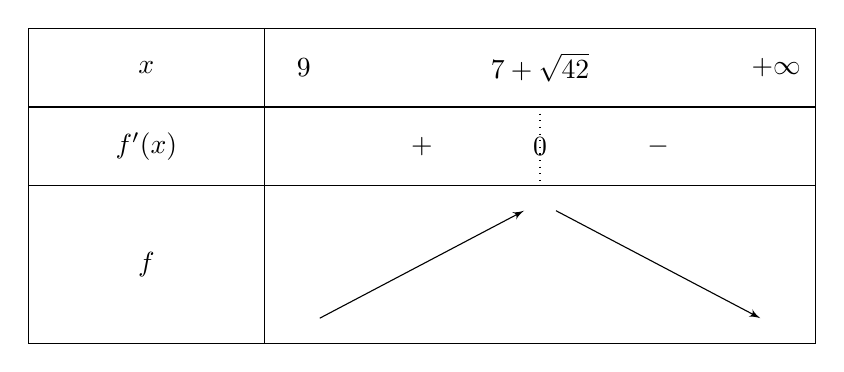
\begin{tikzpicture}[scale=1]
\tikzset{node style/.style = {inner sep = 2pt, outer sep = 2pt}}
   \tkzTabInit[lgt=3]{$x$ / 1 , $f'(x)$/1, $f$ / 2}{$9$,  $7+\sqrt{42}$,$+\infty$}
   \tkzTabLine{, +, z, -, }
   \tkzTabVar{-/$ $,+/$ $,-/$ $}
\end{tikzpicture}\end{center}

La fonction $f$ atteint donc son maximum en $7+\sqrt{42}$ soit environ 13,48.

Or, nous recherchons un entier. On teste alors les valeurs $n=13$ et $n=14$ et on calcule l'espérance dans chacun des cas.
\begin{itemize}
\item Si $n=13$, on a $E[X]= \dfrac{20}{13}$.
\item Si $n=14$, on a $E[X]=\dfrac{20}{13}$.
\end{itemize}

L'espérance de $X$ est donc maximale si l'on place 6 ou 7 jetons dans l'urne.

\end{solution}



\section*{Exercices de synthèse}

\begin{exercise}[subtitle={(Centres étrangers 2022)}]
Une urne contient des jetons blancs et noirs tous indiscernables au toucher.

Une partie consiste à prélever au hasard successivement et avec remise deux jetons de cette urne. On établit la règle de jeu suivante :
\begin{itemize}
\item un joueur perd 9 euros si les deux jetons tirés sont de couleur blanche ;
\item un joueur perd 1 euro si les deux jetons tirés sont de couleur noire ;
\item un joueur gagne 5 euros si les deux jetons tirés sont de couleurs différentes.
\end{itemize}

\begin{enumerate} 
\item On considère que l'urne contient 2 jetons noirs et 3 jetons blancs.
 \begin{enumerate}
\item Modéliser la situation à l'aide d'un arbre pondéré.
\item Calculer la probabilité de perdre 9 euros sur une partie.\end{enumerate}
\item On considère maintenant que l'urne contient 3 jetons blancs et au moins deux jetons noirs
mais on ne connait pas le nombre exact de jetons noirs. On appellera $N$ le nombre de jetons
noirs.
\begin{enumerate} \item Soit $X$ la variable aléatoire donnant le gain du jeu pour une partie.
Déterminer la loi de probabilité de cette variable aléatoire.
\item Résoudre l'inéquation pour $x$ réel : $-x^2+30x-81>0$
\item En utilisant le résultat de la question précédente, déterminer le nombre de jetons noirs
que l'urne doit contenir afin que ce jeu soit favorable au joueur.
\item Combien de jetons noirs le joueur doit-il demander afin d'obtenir un gain moyen maximal ?\end{enumerate}\end{enumerate}\end{exercise}

\begin{solution}\hspace{0pt}


\begin{enumerate} 
\item 
\begin{enumerate}
\item On modélise la situation à l'aide de l'arbre pondéré suivant



\tikzstyle{level 1}=[level distance=3.5cm, sibling distance=3cm]
\tikzstyle{level 2}=[level distance=3.5cm, sibling distance=1.5cm]
\tikzstyle{level 3}=[level distance=3.5cm, sibling distance=0.3cm]

% Define styles for bags and leafs
\tikzstyle{bag} = []
\tikzstyle{end} = [circle, minimum width=3pt,fill, inner sep=0pt]


\begin{center}
\begin{tikzpicture}[scale=0.8,grow=right,sloped]
\node[bag] { }
	child {
        node[bag] {$N$} 
        child {
                node[bag] {$N$}
                edge from parent node[below] {$0.4$}
            }
        child {
               node[bag] {$B$}
               edge from parent node[above] {$0.6$}
            }
            edge from parent node[below] {$0.4$}
    }
	child {
        node[bag] {$B$} 
        child {
                node[bag] {$N$}
                edge from parent node[below] {$0.4$}
            }
        child {
               node[bag] {$B$}
               edge from parent node[above] {$0.6$}
            }
            edge from parent node[above] {$0.6$}
    };
\end{tikzpicture}
\end{center}

\item La probabilité de perdre 9 euros sur une partie correspond au fait de tirer 2 jetons blancs. Ceci arrive avec une probabilité de $0.6 \times 0.6$ soit $0.36$.\end{enumerate}
\item On considère maintenant que l'urne contient 3 jetons blancs et au moins deux jetons noirs
mais on ne connait pas le nombre exact de jetons noirs. On appellera $N$ le nombre de jetons
noirs.
\begin{enumerate} \item Il y a alors 3 jetons blancs, $N$ jetons noirs et donc $N+3$ jetons au total. La probabilité de tirer deux jetons blancs vaut $\dfrac{9}{(N+3)^2}$. \\ La probabilité de tirer deux jetons noirs vaut $\dfrac{N^2}{(N+3)^2}$. La probabilité de tirer deux jetons de couleurs différentes vaut $\dfrac{6N}{(N+3)^2}$ : on tire blanc puis noir ou noir puis blanc : la première possibilité à une probabilité de $\dfrac{3}{N+3} \times \dfrac{N}{N+3}$ et la deuxième a une probabilité de $\dfrac{N}{N+3} \times \dfrac{3}{N+3}$.

On peut alors résumer la loi de $X$ sous la forme d'un tableau.

\begin{center}
\begin{tabular}{|l|c|c|c|c|c|c|}
\hline
$k$ & $-9$ & $-1$ & $5$ \\
\hline
$\mathbb{P}(X=k)$ & $\dfrac{9}{(N+3)^2}$  & $\dfrac{N^2}{(N+3)^2}$&$\dfrac{6N}{(N+3)^2}$\\
\hline \end{tabular}
\end{center}
 

\item Le polynôme  $-x^2+30x-81>0$ possède deux racines qui sont 3 et 27. Le coefficient dominant de ce polynôme est négatif, ainsi, $-x^2+30x-81>0$ si et seulement si $x\in]3;27[$.
\item On a $E(X)=-9\times \dfrac{9}{(N+3)^2}-1 \times \dfrac{N^2}{(N+3)^2}+5 \times \dfrac{6N}{(N+3)^2}=\dfrac{-N^2+30N-81}{(N+3)^2}$. Cette quantité est du signe de $-N^2+30N-81$, qui est strictement positif si et seulement si $3<N<27$. $N$ étant un entier, le jeu est favorable au joueur si le jeu présente entre 4 et 26 boules noirs (4 et 26 inclus).
\item On considère la fonction $f:x\mapsto  \dfrac{-x^2+30x-81}{(x+3)^2}$, définie sur $[0;+\infty[$. $f$ est dérivable sur cet intervalle et, pour tout réel $x\geqslant 0$, \[f'(x)=\dfrac{(-2x+30)(x+3)^2-2(x+3)(-x^2+30x+81)}{((x+3)^2)^2}=\dfrac{-2x^2-6x+30x+90+2x^2-60x+162}{(x+3)^4}\]
Ainsi, pour tout réel $x$, $f'(x)=\dfrac{-36x+252}{(x+3)^4}$. $f'(x)$ est du signe de $-36x+252$. \\
Or, $-36x+252>0$ si et seulement si $x<7$. Ainsi, $f$ est croissante sur $[0;7]$ puis décroissante sur $[7;+\infty[$. Elle admet donc un maximum en 7. L'espérance de gain du joueur est donc maximal lorsqu'il y a 7 boules noires dans l'urne.
\end{enumerate}\end{enumerate}\end{solution}







\begin{exercise}[subtitle={(Métropole 2022)}] Un hôtel situé à proximité d'un site touristique dédié à la préhistoire propose deux visites dans
les environs, celle d'un musée et celle d'une grotte.
Une étude a montré que 70\% des clients de l'hôtel visitent le musée. De plus, parmi les clients
visitant le musée, 60\% visitent la grotte.
Cette étude montre aussi que 6\% des clients de l'hôtel ne font aucune visite.
On interroge au hasard un client de l'hôtel et on note :
\begin{itemize}
\item $M$ l'évènement : « le client visite le musée » ;
\item $G$ l'évènement : « le client visite la grotte ».\end{itemize}
On note $\overline{M}$ l'évènement contraire de $M$, $\overline{G}$ l'évènement contraire de $G$, et pour tout évènement $E$, on note $p(E)$ la probabilité de $E$. Ainsi, d'après l'énoncé, on a : $p(M\cap G)=0.06$.

\begin{enumerate}\item \begin{enumerate}
\item Vérifier que $p_{\overline{M}}(\overline{G})=0.2$, où $p_{\overline{M}}(\overline{G})$ désigne la probabilité que le client interrogé ne visite pas la grotte sachant qu'il
ne visite pas le musée.
\item L'arbre pondéré ci-dessous modélise la
situation. Compléter cet
arbre en indiquant sur chaque branche
la probabilité associée.

\begin{center}

\tikzstyle{level 1}=[level distance=3.5cm, sibling distance=2cm]
\tikzstyle{level 2}=[level distance=3.5cm, sibling distance=1cm]
\tikzstyle{level 3}=[level distance=3.5cm, sibling distance=0.3cm]

% Define styles for bags and leafs
\tikzstyle{bag} = [text width=4em, text centered]
\tikzstyle{end} = [circle, minimum width=3pt,fill, inner sep=0pt]

\begin{tikzpicture}[scale=0.8,grow=right,sloped]
\node[bag] { }
	child {
        node[bag] {$\overline{M}$} 
        child {
                node[bag] {$\overline{G}$}
            }
        child {
               node[bag] {$G$}
            }
    }
	child {
        node[bag] {$M$} 
        child {
                node[bag] {$\overline{G}$}
            }
        child {
               node[bag] {$G$}
            }
    };
\end{tikzpicture}
\end{center}

\item Quelle est la probabilité de l'évènement
« le client visite la grotte et ne visite pas
le musée » ?
\item Montrer que $p(G) = 0,66$.
\end{enumerate}
\item Le responsable de l'hôtel affirme que parmi les clients qui visitent la grotte, plus de la moitié
visitent également le musée. Cette affirmation est-elle exacte ?
\item Les tarifs pour les visites sont les suivants :
\begin{itemize}
\item visite du musée : 12 euros ;
\item visite de la grotte : 5 euros.\end{itemize}
On considère la variable aléatoire $T$ qui modélise la somme dépensée par un client de l'hôtel pour ces visites.
\begin{enumerate}
\item Donner la loi de probabilité de $T$. On présentera les résultats sous la forme d'un tableau.
\item Calculer l'espérance mathématique de T.
\item Pour des questions de rentabilité, le responsable de l'hôtel estime que le montant
moyen des recettes des visites doit être supérieur à 700 euros par jour.
Déterminer le nombre moyen de clients par journée permettant d'atteindre cet objectif.\end{enumerate}
\item Pour augmenter les recettes, le responsable souhaite que l'espérance de la variable aléatoire modélisant la somme dépensée par un client de l'hôtel pour ces visites passe à 15 euros, sans modifier le prix de visite du musée qui demeure à 12 euros.
Quel prix faut-il fixer pour la visite de la grotte afin d'atteindre cet objectif ? (On admettra
que l'augmentation du prix d'entrée de la grotte ne modifie pas la fréquentation des deux
sites).\end{enumerate}\end{exercise}

\begin{solution}\hspace{0pt}

\begin{enumerate}\item \begin{enumerate}
\item On a $p_{\overline{M}}(\overline{G})=\dfrac{p(\overline{M} \cap \overline{G})}{p(\overline{M})}$. Or, 6\% des clients ne font aucune visite. Ainsi, $p(\overline{M} \cap \overline{G})=0.06$. \\De plus, 70\% des clients visitent le musée. Ainsi, $p(M)=0.7$ et $p(\overline{M})=1-0.7=0.3$. \\Finalement, $p_{\overline{M}}(\overline{G})=\dfrac{0.06}{0.3}=0.2$.
\item L'arbre pondéré ci-dessous modélise la
situation.

\begin{center}

\tikzstyle{level 1}=[level distance=3.5cm, sibling distance=2cm]
\tikzstyle{level 2}=[level distance=3.5cm, sibling distance=1cm]
\tikzstyle{level 3}=[level distance=3.5cm, sibling distance=0.3cm]

% Define styles for bags and leafs
\tikzstyle{bag} = [text width=4em, text centered]
\tikzstyle{end} = [circle, minimum width=3pt,fill, inner sep=0pt]

\begin{tikzpicture}[scale=0.8,grow=right,sloped]
\node[bag] { }
	child {
        node[bag] {$\overline{M}$} 
        child {
                node[bag] {$\overline{G}$}
                edge from parent node[above] {$0.2$}
            }
        child {
               node[bag] {$G$}
               edge from parent node[above] {$0.8$}
            }
            edge from parent node[above] {$0.3$}
    }
	child {
        node[bag] {$M$} 
        child {
                node[bag] {$\overline{G}$}
                edge from parent node[above] {$0.4$}
            }
        child {
               node[bag] {$G$}
               edge from parent node[above] {$0.6$}
            }
            edge from parent node[above] {$0.7$}
    };
\end{tikzpicture}
\end{center}

\item On a $p(\overline{M}\cap G)=p(\overline{M}) \times p_{\overline{M}}(G)=0.3 \times 0.8 = 0.24$. 
\item $(M,\overline{M})$ forme un système complet d'événements. D'après la formule des probabilités totales, $p(G)=p(\overline{M} \cap G)+p(M\cap G)=0.24+0.7 \times 0.6=0.66$. 
\end{enumerate}
\item On a $p_G(M)=\dfrac{p(G\cap M)}{p(G)}=\dfrac{0.42}{0.66}\simeq 0.64>0.5$. L'affirmation du responsable de l'hôtel est exacte.
\item 
\begin{enumerate}
\item La loi de probabilité de $T$ est la suivante.

\begin{center}
\begin{tabular}{|l|c|c|c|c|}
\hline
Événement & $M \cap G$ & $\overline{M}\cap G$ & $M \cap \overline{G}$ &$\overline{M} \cap \overline{G}$ \\
\hline
Dépense & $17$ & $5$ & $12$ & $0$ \\
\hline
$\mathbb{P}(X=k)$ & $0.42$  & $0.24$&$0.28$ & $0.06$\\
\hline \end{tabular}
\end{center}

\item On a $E(T)=17 \times 0.42 + 5 \times 0.24 + 12 \times 0.28 + 0 \times 0.06 = 11.7$.
\item Chaque visiteur dépense en moyenne $11.7$ euros. Il faut donc que le nombres $x$ de visiteurs doit tel que $11.7x \geqslant 700$, soit $x \geqslant \dfrac{700}{11.7}\simeq 59.8$. Il faut donc atteindre au moins 60 visiteurs.\end{enumerate}
\item Notons $x$ le prix de la visite de la grotte. La loi de $T$ est alors la suivante.

\begin{center}
\begin{tabular}{|l|c|c|c|c|}
\hline
Événement & $M \cap G$ & $\overline{M}\cap G$ & $M \cap \overline{G}$ &$\overline{M} \cap \overline{G}$ \\
\hline
Dépense& $12+x$ & $x$ & $12$ & $0$ \\
\hline
$\mathbb{P}(X=k)$ & $0.42$  & $0.24$&$0.28$ & $0.06$\\
\hline \end{tabular}
\end{center}

Son espérance vaut alors $E(T)=(12+x) \times 0.42 + x \times 0.24 + 12 \times 0.28 + 0 \times 0.06 = 0.66x+8.4$. Or, $8.4x+0.66\geqslant 15$ si et seulement si $x\geqslant 10$. Le prix de la visite de la grotte doit être fixée à 10 euros.\end{enumerate}\end{solution}




\chapter{Corrigés}


\printsolutions[headings={false} ]





\end{document}